% Options for packages loaded elsewhere
\PassOptionsToPackage{unicode}{hyperref}
\PassOptionsToPackage{hyphens}{url}
%
\documentclass[
  english,
  man,floatsintext]{apa6}
\usepackage{amsmath,amssymb}
\usepackage{lmodern}
\usepackage{ifxetex,ifluatex}
\ifnum 0\ifxetex 1\fi\ifluatex 1\fi=0 % if pdftex
  \usepackage[T1]{fontenc}
  \usepackage[utf8]{inputenc}
  \usepackage{textcomp} % provide euro and other symbols
\else % if luatex or xetex
  \usepackage{unicode-math}
  \defaultfontfeatures{Scale=MatchLowercase}
  \defaultfontfeatures[\rmfamily]{Ligatures=TeX,Scale=1}
\fi
% Use upquote if available, for straight quotes in verbatim environments
\IfFileExists{upquote.sty}{\usepackage{upquote}}{}
\IfFileExists{microtype.sty}{% use microtype if available
  \usepackage[]{microtype}
  \UseMicrotypeSet[protrusion]{basicmath} % disable protrusion for tt fonts
}{}
\makeatletter
\@ifundefined{KOMAClassName}{% if non-KOMA class
  \IfFileExists{parskip.sty}{%
    \usepackage{parskip}
  }{% else
    \setlength{\parindent}{0pt}
    \setlength{\parskip}{6pt plus 2pt minus 1pt}}
}{% if KOMA class
  \KOMAoptions{parskip=half}}
\makeatother
\usepackage{xcolor}
\IfFileExists{xurl.sty}{\usepackage{xurl}}{} % add URL line breaks if available
\IfFileExists{bookmark.sty}{\usepackage{bookmark}}{\usepackage{hyperref}}
\hypersetup{
  pdftitle={English Negative Constructions and Communicative Functions in Early Child Language},
  pdfauthor={Zoey Liu1 \& Masoud Jasbi2},
  pdflang={en-EN},
  pdfkeywords={negation; syntactic construction; communicative function; development; child language.},
  hidelinks,
  pdfcreator={LaTeX via pandoc}}
\urlstyle{same} % disable monospaced font for URLs
\usepackage{longtable,booktabs,array}
\usepackage{calc} % for calculating minipage widths
% Correct order of tables after \paragraph or \subparagraph
\usepackage{etoolbox}
\makeatletter
\patchcmd\longtable{\par}{\if@noskipsec\mbox{}\fi\par}{}{}
\makeatother
% Allow footnotes in longtable head/foot
\IfFileExists{footnotehyper.sty}{\usepackage{footnotehyper}}{\usepackage{footnote}}
\makesavenoteenv{longtable}
\usepackage{graphicx}
\makeatletter
\def\maxwidth{\ifdim\Gin@nat@width>\linewidth\linewidth\else\Gin@nat@width\fi}
\def\maxheight{\ifdim\Gin@nat@height>\textheight\textheight\else\Gin@nat@height\fi}
\makeatother
% Scale images if necessary, so that they will not overflow the page
% margins by default, and it is still possible to overwrite the defaults
% using explicit options in \includegraphics[width, height, ...]{}
\setkeys{Gin}{width=\maxwidth,height=\maxheight,keepaspectratio}
% Set default figure placement to htbp
\makeatletter
\def\fps@figure{htbp}
\makeatother
\setlength{\emergencystretch}{3em} % prevent overfull lines
\providecommand{\tightlist}{%
  \setlength{\itemsep}{0pt}\setlength{\parskip}{0pt}}
\setcounter{secnumdepth}{-\maxdimen} % remove section numbering
% Make \paragraph and \subparagraph free-standing
\ifx\paragraph\undefined\else
  \let\oldparagraph\paragraph
  \renewcommand{\paragraph}[1]{\oldparagraph{#1}\mbox{}}
\fi
\ifx\subparagraph\undefined\else
  \let\oldsubparagraph\subparagraph
  \renewcommand{\subparagraph}[1]{\oldsubparagraph{#1}\mbox{}}
\fi
% Manuscript styling
\usepackage{upgreek}
\captionsetup{font=singlespacing,justification=justified}

% Table formatting
\usepackage{longtable}
\usepackage{lscape}
% \usepackage[counterclockwise]{rotating}   % Landscape page setup for large tables
\usepackage{multirow}		% Table styling
\usepackage{tabularx}		% Control Column width
\usepackage[flushleft]{threeparttable}	% Allows for three part tables with a specified notes section
\usepackage{threeparttablex}            % Lets threeparttable work with longtable

% Create new environments so endfloat can handle them
% \newenvironment{ltable}
%   {\begin{landscape}\begin{center}\begin{threeparttable}}
%   {\end{threeparttable}\end{center}\end{landscape}}
\newenvironment{lltable}{\begin{landscape}\begin{center}\begin{ThreePartTable}}{\end{ThreePartTable}\end{center}\end{landscape}}

% Enables adjusting longtable caption width to table width
% Solution found at http://golatex.de/longtable-mit-caption-so-breit-wie-die-tabelle-t15767.html
\makeatletter
\newcommand\LastLTentrywidth{1em}
\newlength\longtablewidth
\setlength{\longtablewidth}{1in}
\newcommand{\getlongtablewidth}{\begingroup \ifcsname LT@\roman{LT@tables}\endcsname \global\longtablewidth=0pt \renewcommand{\LT@entry}[2]{\global\advance\longtablewidth by ##2\relax\gdef\LastLTentrywidth{##2}}\@nameuse{LT@\roman{LT@tables}} \fi \endgroup}

% \setlength{\parindent}{0.5in}
% \setlength{\parskip}{0pt plus 0pt minus 0pt}

% \usepackage{etoolbox}
\makeatletter
\patchcmd{\HyOrg@maketitle}
  {\section{\normalfont\normalsize\abstractname}}
  {\section*{\normalfont\normalsize\abstractname}}
  {}{\typeout{Failed to patch abstract.}}
\patchcmd{\HyOrg@maketitle}
  {\section{\protect\normalfont{\@title}}}
  {\section*{\protect\normalfont{\@title}}}
  {}{\typeout{Failed to patch title.}}
\makeatother
\shorttitle{Negation and communicative functions}
\keywords{negation; syntactic construction; communicative function; development; child language.
\newline\indent Word count: X}
\usepackage{lineno}

\linenumbers
\usepackage{csquotes}
\ifxetex
  % Load polyglossia as late as possible: uses bidi with RTL langages (e.g. Hebrew, Arabic)
  \usepackage{polyglossia}
  \setmainlanguage[]{english}
\else
  \usepackage[main=english]{babel}
% get rid of language-specific shorthands (see #6817):
\let\LanguageShortHands\languageshorthands
\def\languageshorthands#1{}
\fi
\ifluatex
  \usepackage{selnolig}  % disable illegal ligatures
\fi
\newlength{\cslhangindent}
\setlength{\cslhangindent}{1.5em}
\newlength{\csllabelwidth}
\setlength{\csllabelwidth}{3em}
\newenvironment{CSLReferences}[2] % #1 hanging-ident, #2 entry spacing
 {% don't indent paragraphs
  \setlength{\parindent}{0pt}
  % turn on hanging indent if param 1 is 1
  \ifodd #1 \everypar{\setlength{\hangindent}{\cslhangindent}}\ignorespaces\fi
  % set entry spacing
  \ifnum #2 > 0
  \setlength{\parskip}{#2\baselineskip}
  \fi
 }%
 {}
\usepackage{calc}
\newcommand{\CSLBlock}[1]{#1\hfill\break}
\newcommand{\CSLLeftMargin}[1]{\parbox[t]{\csllabelwidth}{#1}}
\newcommand{\CSLRightInline}[1]{\parbox[t]{\linewidth - \csllabelwidth}{#1}\break}
\newcommand{\CSLIndent}[1]{\hspace{\cslhangindent}#1}

\title{English Negative Constructions and Communicative Functions in Early Child Language}
\author{Zoey Liu\textsuperscript{1} \& Masoud Jasbi\textsuperscript{2}}
\date{}


\authornote{

Add complete departmental affiliations for each author here. Each new line herein must be indented, like this line.

Enter author note here.

Correspondence concerning this article should be addressed to Zoey Liu, . E-mail:

}

\affiliation{\vspace{0.5cm}\textsuperscript{1} Boston College\\\textsuperscript{2} UC Davis}

\abstract{
How does abstract linguistic negation develop in early child language? Previous research has suggested that abstract negation develops in stages and from more concrete communicative functions such as rejection, prohibition, or non-existence. The evidence for the emergence of these functions in stages is mixed, however, leaving the possibility that negation is an abstract concept from the beginning that can serve multiple specific functions depending on early communicative environment. Leveraging automatic annotations of large-scale child speech corpora in English, we examine the production trajectores of seven negative constructions that tend to convey communicative functions previously discussed in the literature. The results demonstrate the emergence and gradual increase of these constructions in child speech within the age range of 18-36 months. Production mostly remains stable, regular, and close to parents' levels after this age range. These findings are consistent with two hypotheses: first, that negation starts as an abstract concept that can serve multiple functions from the beginning; and second, that negation develops in stages from specific communicative functions but this development is early and quick, leaving our corpus methods incapable of detecting them from the available corpus data.
}



\begin{document}
\maketitle

\hypertarget{introduction}{%
\section{Introduction}\label{introduction}}

Negation is an abstract concept that serves different communicative functions in everyday communication. A coffee shop can divide its menu into ``coffee'' and ``not coffee'' sections, with ``not coffee'' bringing together diverse items with no common label like tea and hot chocolate. It could be used in a sign like ``no mask, no entry'' to regulate people's behaviors. An employee could say ``I don't like Mondays'' to communicate their desires or dislikes. But how does abstract multi-functional negation emerge and develop in the human mind? Are early stages of negation in child language specific to one or a few functions? Or does negation emerge as an abstract and multifunctional concept from the beginning?

Previous literature has proposed that abstract negation develops from less abstract communicative functions in ordered stages (Pea, 1978). For instance, Darwin (1872) hypothesized that the earliest manifestation of negation in infants is when they refuse or reject food from parents by withdrawing their heads laterally. Similarly, Pea (1978) also proposed ``rejection'' as the first function of negation in child language. By contrast, Bloom (1970) argued that the use of negation to express ``non-existence'' emerges before ``rejection.'' For example, when an object that children expect to be present is not, children may say: ``there is no window.'' Follow-up study by Choi (1988) argued that ``prohibition'' emerges as early as rejections and non-existence. In cases of prohibition, children use negation to stop others or themselves from performing actions (e.g.~``don't go''). A function similar to prohibition is ``inability'' (e.g.~``I cannot zip it''), in that both involve conceptualizing actions and negating them. Choi (1988) suggested that expressions of inability emerge after the functions in the first phase, namely non-existence, rejection, and prohibition.

Despite considerable research on early communicative functions of negation, their developmental trajectories in children's production have remained unclear. Recently, Nordmeyer and Frank (2018) looked at the speech of five children in the Providence corpus (Demuth, Culbertson, \& Alter, 2006) and found a great deal of individual variation in how early a negative function is attested. They reported that the
developmental trajectory of negation in their study was not as consistent as previously claimed. This leaves the possibility that negation develops as an abstract concept that can serve multiple communicative functions early in the development based on the context of use in parent-child interactions. Therefore, across (a larger number of) children, distinct functions of negation could develop within the same age range and share common production trajectories.

However, previous experiments have mainly relied on manual annotations of corpus data to determine the communicative function of a given negative utterance, which in turn has limited their work to only a handful of children per study.
Here we aim to go beyond existing work via utilizing a large collection of child speech corpora in English (MacWhinney, 2000) along with computational tools to automatically identify negative utterances that tend to convey the communicative functions discussed in prior research (Table 1). In particular, our study investigates three questions: (1) how does the developmental trajectory of the negative constructions for each function look like? (2) for utterances expressing the same function, does the developmental trajectory differ depending on particular lexical items that negation modifies (e.g.~\emph{like} or \emph{want} for rejection)? (3) taking all functions into account, do they share similar developmental characteristics, or would there be function-specific differences?

Given the automatic fashion of our approach, we focus on larger/longer negative constructions at the single-sentence level. This is in opposition to short negative forms at the discourse-level such as cases consisting of one morpheme (e.g.~``no!'') or repetition of negative morphemes (e.g.~``no no no''), which arguably could express multiple functions when not taking the discourse context into account and accordingly leave more room for ambiguous interpretation. Therefore the negative utterances in our study do not fully cover all negation instances from the corpora investigated, nor reflect all possible communicative functions that could be played by negation more broadly, but it could provide at least a conservative estimate of the age range during which negation is developed gradually in child production.

\begin{table*}[h]
\small
\centering
\begin{tabular}{rrrr}
  \hline
 \textbf{Function} & \textbf{Linguistic Composition} & \textbf{Examples} & \textbf{Positive counterpars} \\
  \hline
Rejection & with \textit{like} or \textit{want} & \textit{I not like it}; \textit{not want it}  & \textit{I like that}; \textit{You want this} \\
Non-existence & expletives & \textit{there is no soup} & \textit{there are books} \\
Prohibition & with imperative subjectless \textit{do} & \textit{do not spill milk} & \textit{eat it} \\
Inability & with modal \textit{can} & \textit{I cannot zip it} & \textit{She can try} \\
Labeling & modifying nominal or adjectival predicatives & \textit{that's not a crocodile}; \textit{it's no interesting} & \textit{that's a table}; \textit{it's cool} \\
Epistemic negation & with \textit{know}, \textit{think}, \textit{remember}  & \textit{I not know/think/remember} & \textit{He knows/thinks/remembers that} \\
Possession & with \textit{have}; or possesive pronouns & \textit{not have the toy}; \textit{not mine} & \textit{have the water}; \textit{theirs} \\
   \hline
\end{tabular}
\caption{Communicative functions of negation in early child language of English.}
\end{table*}

\hypertarget{related-work}{%
\section{Related Work}\label{related-work}}

Starting a century and a half ago, Darwin (1872) thought that negation has roots in the expression of human emotions and desires. He hypothesized the earliest manifestation of negation and affirmation in infants is when they refuse food from parents, by withdrawing their heads laterally, or when they accept the food, by inclining their heads forward. He suggested that head shaking and nodding as common gestures for negation and affirmation pro developed from this early habit. Similarly, many researchers studying early functions of negative morphemes like \emph{no} proposed that children use them to ``reject'' or ``refuse'' (Bloom, 1970; Choi, 1988; Pea, 1978). For example, when they are asked ``do you want juice?'' they may say ``no,'' ``not want it,'' or ``don't like it.'' Pea (1978) proposed this negation function is the first to emerge in children's early speech.

Bloom (1970) argued that the use of negation to expresses ``non-existence'' emerges before rejection or refusal. For example, when an object that children expect to be present is not present, children may say: ``no window,'' ``no fish in the bathroom,'' or ``I do not pro underpants.'' Two close concepts to non-existence are ``disappearance'' and ``non-occurrence'' (Pea, 1978; Villiers \& Villiers, 1979). Disappearance refers to situations where an object disappears and children use negation to express it (e.g.~``no food. all gone'' or ``no more noise''). Non-occurrence refers to cases when an expected action or event does not occur as in ``not working'' or ``doggie not barking.'' Some researchers referred to these cases as ``failures'' and included examples like ``no fit in da box'' or ``it don't fit'' (Cameron-Faulkner, Lieven, \& Theakston, 2007; Choi, 1988). Non-existence can also be expressed by negation of locative prepositional phrases (e.g.~``no in there'' or ``daddy was not on the phone''). While rejection was hypothesized to interact with human emotions and desires, non-existence (broadly construed to include ``disappearance'' and ``non-occurrence'') likely interacts with human perception. Choi (1988) proposed that children's early linguistic negation is used to express both rejection and non-existence.

Additionally, Choi (1988) introduced ``prohibition'' and suggested that it emerges as early as rejection and non-existence. In cases of prohibition, children use negation to stop others from performing actions; for example ``don't go'' or ``do not spill milk.'' A special case of prohibition is ``self-prohibition.'' For example, a child may approach prohibited food but immediately say ``no, don't eat'' to stop themselves. A function similar to prohibition is ``inability'' (e.g.~\emph{I can't reach} / \emph{I cannot zip it}), in that both involve conceptualizing actions and negating them, possibly interacting with early development of motor control. Choi (1988) suggested that expression of inability emerges after the first phase, namely non-existence, rejection, and prohibition.

``Denial'' is another function of negation that is argued to be late in development. Bloom (1970) defined it as asserting that ``an actual or supposed predication was not the case,'' for example ``It's not sharp.'' Later researchers formulated it as ``truth-functional negation'' because it is used to negate the truth of a proposition (Cameron-Faulkner, Lieven, \& Theakston, 2007; Pea, 1978). However, this definition depends on the assumed logical system and its assumptions on what type of propositions receive truth values. A particular sub-function of denial is ``labeling,'' which is realized as the negation of nominal or adjectival predicates such as ``this is not a bunny'' or ``not red.'' These utterances are often used to introduce new linguistic labels by parents and in turn may facilitate word learning (Clark, 2010). Conversely, labeling and word learning may aid the development of abstract negation.

Despite considerable research on early functions of negation, their developmental trajectories in children's productions pro remained unclear. Different studies pro claimed different order of acquisition (Pea, 1978). In a recent study, Nordmeyer and Frank (2018) looked at the speech of five children in the Providence corpus (Demuth, Culbertson, \& Alter, 2006) and found a great deal of individual differences in how early a negative function is attested. This is partly because previous studies pro had to rely on human annotation and identification of functions from corpus data, a time-consuming and difficult process that has limited previous studies to a handful of children and a relatively small sample of their speech.

\hypertarget{experiments}{%
\section{Experiments}\label{experiments}}

\hypertarget{data-and-preprocessing}{%
\subsection{Data and preprocessing}\label{data-and-preprocessing}}

For child language data, we turned to the CHILDES database (MacWhinney, 2000)\footnote{Code and data are in quarantine at \url{https://github.com/zoeyliu18/Negative_Constructions.}} and selected English speaking children with typical development within the age range of 12 - 72 months. Parents' and children's utterances were extracted via the childes-db (Sanchez et al., 2019) interface using the programming language R. In order to obtain (morpho)syntactic representations for parents' and children's utterances, we used the dependency grammar framework (Tesnière, 1959). Part-of-speech (POS) tags for each token within an utterance were automatically derived using Stanza (Qi, Zhang, Zhang, Bolton, \& Manning, 2020), an open-source natural language processing library; dependency relations for all utterances were acquired also in an automatic fashion using DiaParser (Attardi, Sartiano, \& Yu, n.d.), a dependency parsing system that has been demonstrated to achieve excellent performance for at least written texts in English.

We focus on seven negative constructions shown in Table 1 that tend to convey the communicative functions of rejection, non-existence, prohibition, inability, labeling, epistemic state, and possession. We test children's knowledge of these constructions at two levels: sentence level and discourse level. Negation is marked in two fundamentally different ways in English and many other languages. First, at sentence level, morphemes such as \emph{no}, \emph{not}, or the reduced form \emph{n't} combine with other lexical items to form a negative sentence. For example in sentence level rejection, \emph{n't} can combine with \emph{want} to form ``\emph{I don't want to go}.'' Second, negative response particles such as \emph{no} can be used anaphorically to negate a previous utterance in discourse. For example in discourse level rejection, when a parent asks ``\emph{Do you want to go?}'' a child can respond with \emph{No!}. Here, the negative discourse particle stands for the proposition ``I don't want to go.'' Children's earliest negative productions are dominated by discourse level negation, presumably because it is shorter and easier to produce when children are limited in their productive capacity. Nevertheless, successful communication with discourse level negation can indicate the children understand the propositions conveyed it.

At the sentence level, we characterized the syntactic features of the negative utterances associated with each communicative function, then classified utterances based on these features in a rule-based fashion with the help of POS information and syntactic dependencies. To decouple the development of the syntactic construction from the development of negation in that construction, we also examined the production of positive counterparts to each negative construction. The positive counterpart of our negative constructions share the same syntactic features (e.g.~same head verb) but they have no negative morphemes. These positive constructions do not express the same communicative function as their negative counterparts. Our main purpose for including the positive counterparts is to factor in the development of the syntactic construction without negation.

At the discourse level, we need to analyze the negative constructions that the discourse particle \emph{No} stands for. To achieve this, we selected utterances that started with negative discourse particles like ``no no I like it.'' These instances were tagged with the dependency relation ``discourse'' by our dependency parser. For each negative utterance identified this way, we extracted the previous utterance (the antecedent) in the discourse context. For child speech, we included interactions (negative utterances + their antecedents) where antecedents were produced by either the parents or the children themselves. For parent speech, we only included interactions where the antecedent was produced by children. We then applied the same analyses we had performed to sentence level constructions to these antecedent utterances. The assumption here is that the negative discourse particles are implicitly negating the content of their discourse antecedents.

\hypertarget{measures}{%
\subsection{Measures}\label{measures}}

We took age as a proxy for children's development and divided the 12-72 months range into monthly bins. We used the following two metrics for each age bin and communicative function. First, we defined the ratio \(R_{c,i}\) for construction \(c\) and age bin \(i\) as the number of utterances in construction \(c\) and age bin \(i\) divided by the total number of utterances produced at age bin \(i\). For example at age 30 months, children produced a total of 81,302 utterances, out of which 391 were classified as rejections. Therefore the ratio of rejection at 30 months is 391/81,302 = 0.005.

\(R_{c, i} = \frac{\#U_{c,i}}{\#U_{i}}\)

Second, we borrowed the measure of ``moving (cumulative) ratio'' from the analysis of time series data (Wei, 2006). We defined the cumulative ratio \(MR_{c,i}\) for a construction \(c\) at age bin \(i\), as the sum of the number of utterances produced with construction \(c\) from the first age bin to age bin \(i\), divided by the sum of all utterances produced between the first age bin and age bin \(i\). For example up to age 30 months, children in our corpus produced 721,748 total utterances, out of which 2,166 were instances of rejection. Therefore, the cumulative ratio of rejection at age 30 months is 2,166/721,748 = 0.003. The cumulative ratio has the advantage that at each age bin, it takes into account the productions in previous age bins. Assuming that children accumulate linguistic knowledge throughout their development, this measure provides a more realistic and stable measure of children's productive capacity at each age.

\(CR_{c, i} = \frac{\#U_{c,1-t}}{\#U_{1-t}}\)

The two ratios mentioned above were calculated for negative constructions and their positive counterparts at sentence and discourse levels for children as well as parents. In this study we use parents' speech as a benchmark for children's development. Therefore, our figures show children's productions side by side the production of parents at the corresponding age of children. In what follows, we describe in detail the results for each communicative function and its associated negative construction.

\hypertarget{negative-constructions}{%
\subsection{Negative Constructions}\label{negative-constructions}}

\hypertarget{rejection}{%
\subsubsection{Rejection}\label{rejection}}

For instances of ``rejection'' and positive counterparts, we selected utterances in which the lemma of the head verb of the phrase is either \emph{like} or \emph{want}. For negative instances, the head verb is modified by one of the three negative morphemes \emph{no}, \emph{not} or \emph{n't}, whereas cases including the same head verb but without negation were classified as positive. Table \ref{tab:rejection} shows examples of negative utterances including those in which the speakers describe their own desires with or without an auxiliary verb (e.g.~1 and 2), as well as cases that express rhetorical inquiries of desires from one interlocutor to another (e.g.~3), and instances where the speaker is describing the desires of somebody else (e.g.~4). We classified a total of 20,641 negative utterances (child: 9,398; parent: 11,243), and a total of 180,881 negative utterances (child: 63,427; parent: 117,454).

\begin{longtable}[]{@{}ll@{}}
\caption{\label{tab:rejection} Examples of sentence level rejection (negative) and positive counterparts in children's speech}\tabularnewline
\toprule
Rejection (Negative) & Positive Counterpart \\
\midrule
\endfirsthead
\toprule
Rejection (Negative) & Positive Counterpart \\
\midrule
\endhead
\emph{I no like sea} & \emph{she likes cheese} \\
\emph{don't wanna go} & \emph{I want it} \\
\emph{don't you wanna try it} & \emph{I wanna have that} \\
\emph{Sarah doesn't like that either} & \emph{she likes this one} \\
\bottomrule
\end{longtable}

\begin{figure}[H]

{\centering 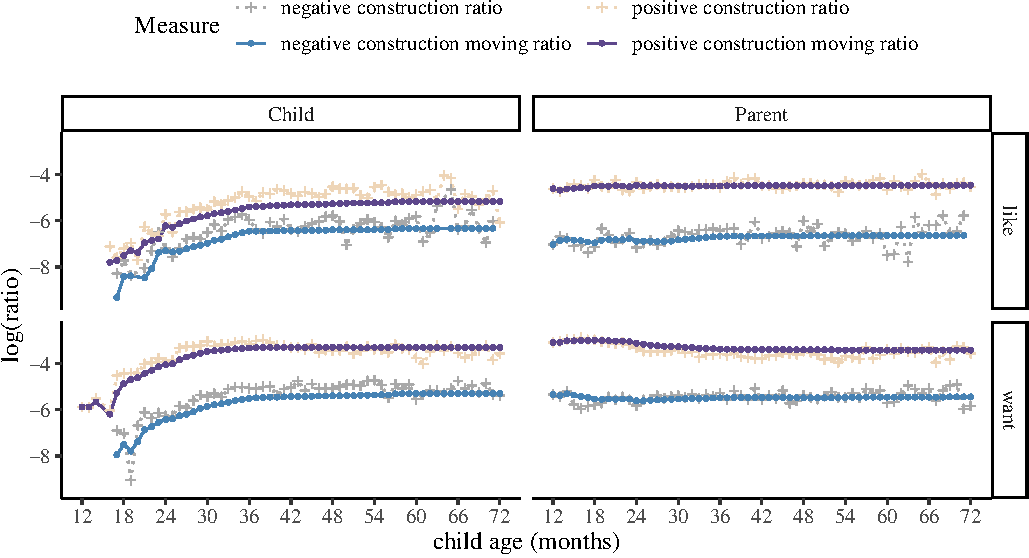
\includegraphics{neg_construction_article_files/figure-latex/emotion-1} 

}

\caption{Rejection and its positive counterparts.}\label{fig:emotion}
\end{figure}

Starting with our analysis at the sentence level, Figure \ref{fig:emotion} shows the ratios and cumulative ratios of parents' and children's instances of rejection and positive counterparts on a logarithmic scale (y-axis) with age along the x-axis. Overall, we see a similar pattern of production for rejection whether the head verb is \emph{want} or \emph{like}. Comparing the cumulative ratios between parents and children, children's production of rejection gradually increases between the ages of 18 and 30 months. After about 30 months of age, children's production of these constructions stays at a relatively constant rate and close to parent levels. In all age bins, the production ratio for negative utterances is lower than that for their positive counterparts.

On the discourse level, we investigated discourse interactions (antecedent + negative utterance) in which the antecedent had one of the head verbs \emph{like} or \emph{want}, yet the head verb did not have to be modified by negative morphemes. Table \ref{tab:disreject} shows a few examples. We found a total of 1,957 such utterances (child: 994; parent: 963). As shown in Figure 2, children's production of negation as discourse response variables increases regularly from the age of 24 - 36 months\footnote{For each communicative function, at the discourse level we also examined cases of different subtypes (e.g. different head verbs) separately; though due to data sparsity issues, we collapsed these instances for our final analyses}. Overall negative morphemes are applied at the discourse level more frequently in child speech compared to parent speech.

\begin{longtable}[]{@{}ll@{}}
\caption{\label{tab:disreject} Example antecdents and discourse level rejections in parents' and children's productions}\tabularnewline
\toprule
Antecedent & Utterance \\
\midrule
\endfirsthead
\toprule
Antecedent & Utterance \\
\midrule
\endhead
Parent: \emph{I want you to try it} & Child: \emph{no no no} \\
Parent: \emph{would you like to go} & Child: \emph{no no} \\
Child: \emph{I don't like that} & Parent: \emph{no honey you have to try it} \\
\bottomrule
\end{longtable}

\begin{figure}[H]

{\centering 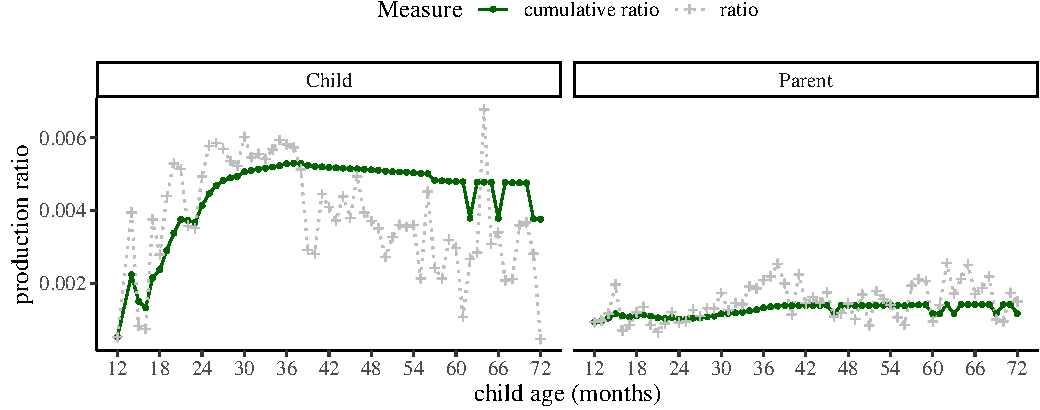
\includegraphics{neg_construction_article_files/figure-latex/emotiondiscourse-1} 

}

\caption{Ratios and cumulative ratios for the production of rejection at the discourse level for children between 1 to 6 years of age, and their parents.}\label{fig:emotiondiscourse}
\end{figure}

\hypertarget{non-existence}{%
\subsubsection{Non-existence}\label{non-existence}}

For this function we searched for the English existential construction and extracted utterances that had \emph{there}-expletives, followed by a copula, and a noun phrase (phrases headed by either nouns or pronouns). We classified utterances where the predicate was modified by negation as negative, and the rest as positive. This led to a total of 1,983 negative utterances (child: 498; parent: 1,485), and a total of 35,287 positive utterances (child: 8,385; parent: 26,902).

\begin{longtable}[]{@{}ll@{}}
\caption{\label{tab:nonexist} Examples of positive and negative existenial constructions in children's speech at the sentence level}\tabularnewline
\toprule
Non-existence (Negative) & Existentials (Positive) \\
\midrule
\endfirsthead
\toprule
Non-existence (Negative) & Existentials (Positive) \\
\midrule
\endhead
\emph{there's no (more) water} & \emph{there are books} \\
\emph{there isn't it} & \emph{there is it} \\
\bottomrule
\end{longtable}

At the sentence level, children produced negative constructions to express non-existence less frequently than the positive counterparts. As Figure \ref{fig:existence} shows, the cumulative ratio for the production of non-existence increases from 18 to 36 months. Around and after 36 months of age, children's productions reaches a stable cumulative ratio close to that of adults. Notice that there appears to be fluctuations of cumulative ratios between the age of 19 and 25 months in child production. A closer inspection of the data reveals that within that age range, the frequency of negative utterances at most ages is either one or zero. Therefore while the number of total utterances increases along the developmental trajectory, the cumulative ratio for negative utterances actually decreases.

\begin{figure}[H]

{\centering 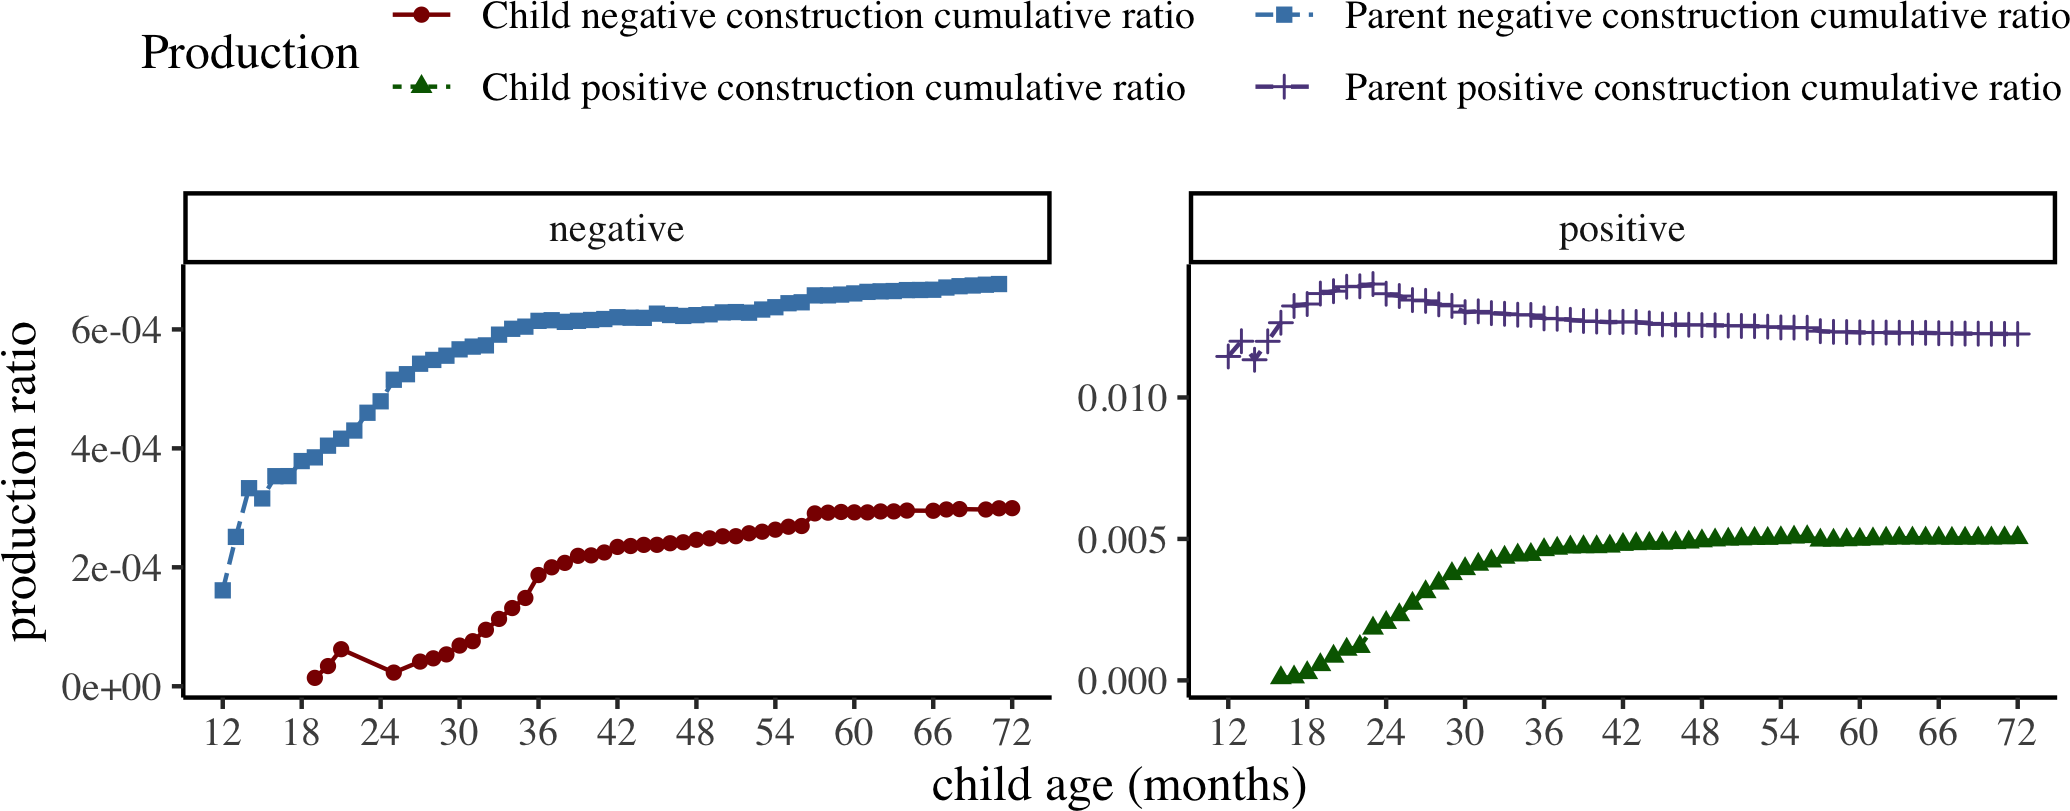
\includegraphics{neg_construction_article_files/figure-latex/existence-1} 

}

\caption{Non-existence and its positive counterparts.}\label{fig:existence}
\end{figure}

For non-existence at the discourse level, we applied similar selection criteria and extracted negative utterances with existential constructions in their antecedents (Table \ref{tab:disexist}). This led to a total of 220 utterances (child: 91; parent: 129). As Figure \ref{fig:exstencediscourse} shows, we could find an increase in children's responses with \emph{no} to parents' existential utterances between the ages of 18 and 36 months. After 36 months, despite the fact that ratios show considerable fluctuations, the cumulative ratios of parents and children seem stable and similar. Therefore with non-existence, both sentence level and discourse level analyses point to substantial development in the age rage of 18-36 months.

\begin{longtable}[]{@{}ll@{}}
\caption{\label{tab:disexist} Example antecedents existentials and discourse level negation in parents' and children's productions}\tabularnewline
\toprule
Antecedent & Utterance \\
\midrule
\endfirsthead
\toprule
Antecedent & Utterance \\
\midrule
\endhead
Parent: \emph{Is there a bunny} & Child: \emph{no no bunny} \\
\bottomrule
\end{longtable}

\begin{figure}[H]

{\centering 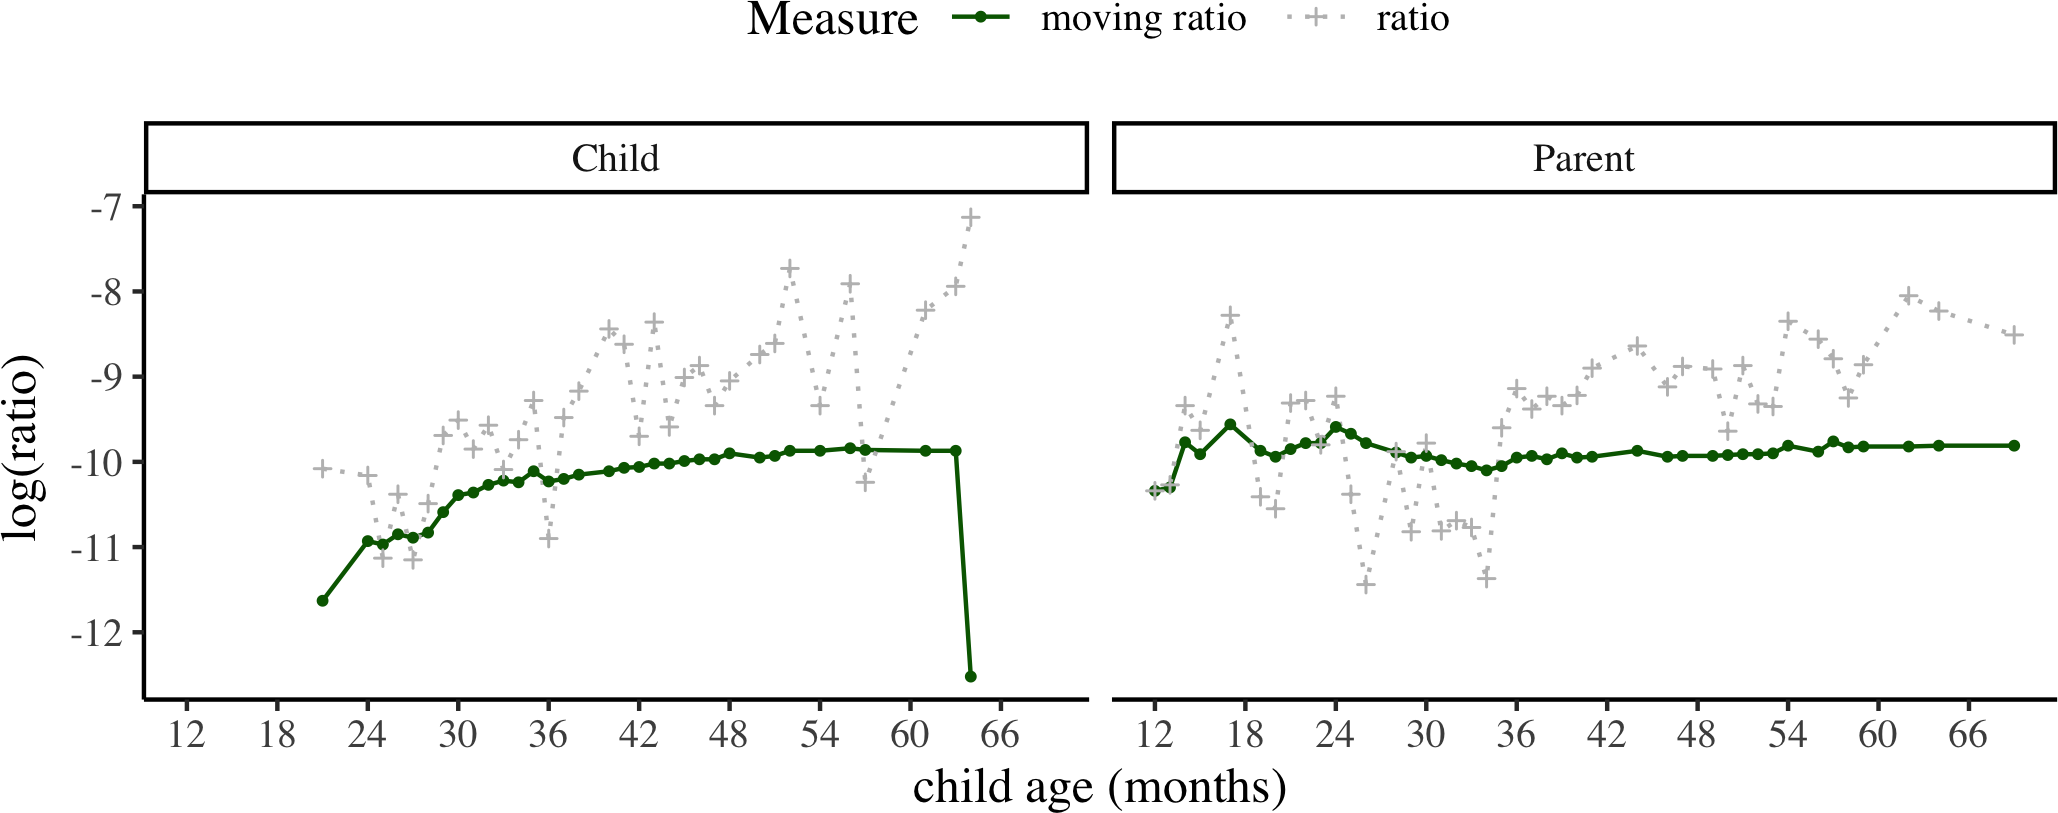
\includegraphics{neg_construction_article_files/figure-latex/existencediscourse-1} 

}

\caption{Discourse-level Non-existence.}\label{fig:existencediscourse}
\end{figure}

\hypertarget{prohibition}{%
\subsubsection{Prohibition}\label{prohibition}}

For constructions that typically convey prohibition, we extracted utterances that were annotated as imperatives in CHILDES. In particular, we selected instances where the head verbs do not take any subjects. As before, cases without any negative morphemes are considered as positive. For negative constructions, we chose structures where the negative morphemes are combined with the auxiliary verb \emph{do} (\emph{do}, \emph{does}, \emph{did}) and they together modify the head verbs of the sentences. In order to not have overlap with rejection, non-existence, epistemic negation and possession (see below), our search excluded utterances where the head verb had any of the following lemma forms: \emph{like}, \emph{want}, \emph{know}, \emph{think}, \emph{remember}, \emph{have}. This resulted in a total of 1,069 negative utterances (child: 309; parent: 760), and a total of 25,542 negative utterances (child: 8,659; parent: 16,883).

Figure \ref{fig:prohibition} shows the ratios and cumulative ratios of prohibitions and their positive counterparts in parents' and children's speech at the sentence level. In both child and parent speech, negative constructions for prohibition are consistently produced less frequently than their positive counterparts. Children produce prohibitions (negative imperatives) more and more often between 24 and 36 months. In comparison, the cumulative ratio in parent speech gradually decreases at the beginning when children between 12 - 36 months. Yet overall, child production is remains consistently lower than parent production of prohibition. This might be due to the social nature of parent-child interactions, in which it is more likely for parents to explicitly command and direct children's actions than the other way round.

\begin{longtable}[]{@{}ll@{}}
\caption{\label{tab:prohibit} Examples of positive and negative imperatives in children's speech at the sentence level}\tabularnewline
\toprule
Prohibition (Negative) & Imperatives (Positive) \\
\midrule
\endfirsthead
\toprule
Prohibition (Negative) & Imperatives (Positive) \\
\midrule
\endhead
\emph{don't blame Charlotte} & \emph{cook it} \\
\bottomrule
\end{longtable}

\begin{figure}[H]

{\centering 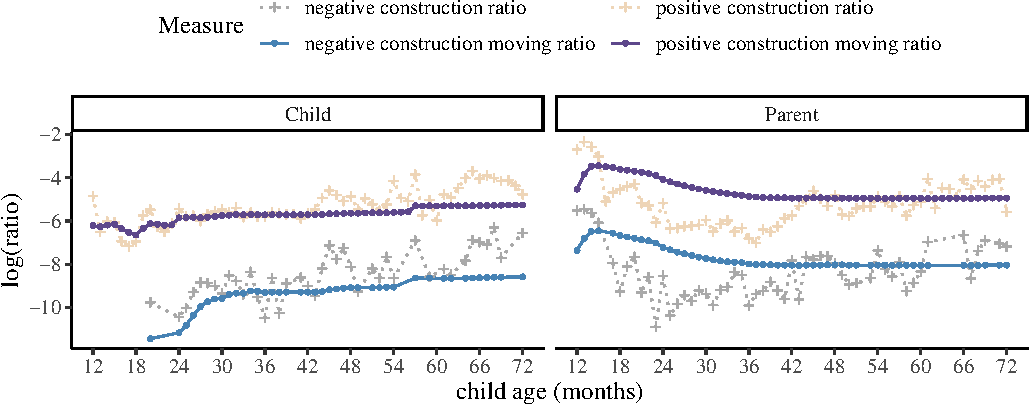
\includegraphics{neg_construction_article_files/figure-latex/prohibition-1} 

}

\caption{Prohibition and its positive counterparts.}\label{fig:prohibition}
\end{figure}

At the discourse level, we selected \emph{No}-utterances with antecedents that were subjectless imperatives headed by a verb, excluding the following lemma forms: \emph{like}, \emph{want}, \emph{know}, \emph{think}, \emph{remember}, nor \emph{have}. This resulted in a total of 238 utterances (child: 8,968; parent: 17,643). As shown in Figure \ref{fig:prohibitiondiscourse}, children's usage of negation as a response particle to express prohibition is comparable to their productions at the sentence level. Their negative productions increases within the age range of 24 to 36 months, and parent production decreases when the children are between 12 to 36 months.

\begin{longtable}[]{@{}ll@{}}
\caption{\label{tab:disprohib} Example antecedents imperatives and discourse level negation in parents' and children's productions}\tabularnewline
\toprule
Antecedent & Utterance \\
\midrule
\endfirsthead
\toprule
Antecedent & Utterance \\
\midrule
\endhead
Parent: \emph{put away your toys} & Child: \emph{no mommy I like these} \\
\bottomrule
\end{longtable}

\begin{figure}[H]

{\centering 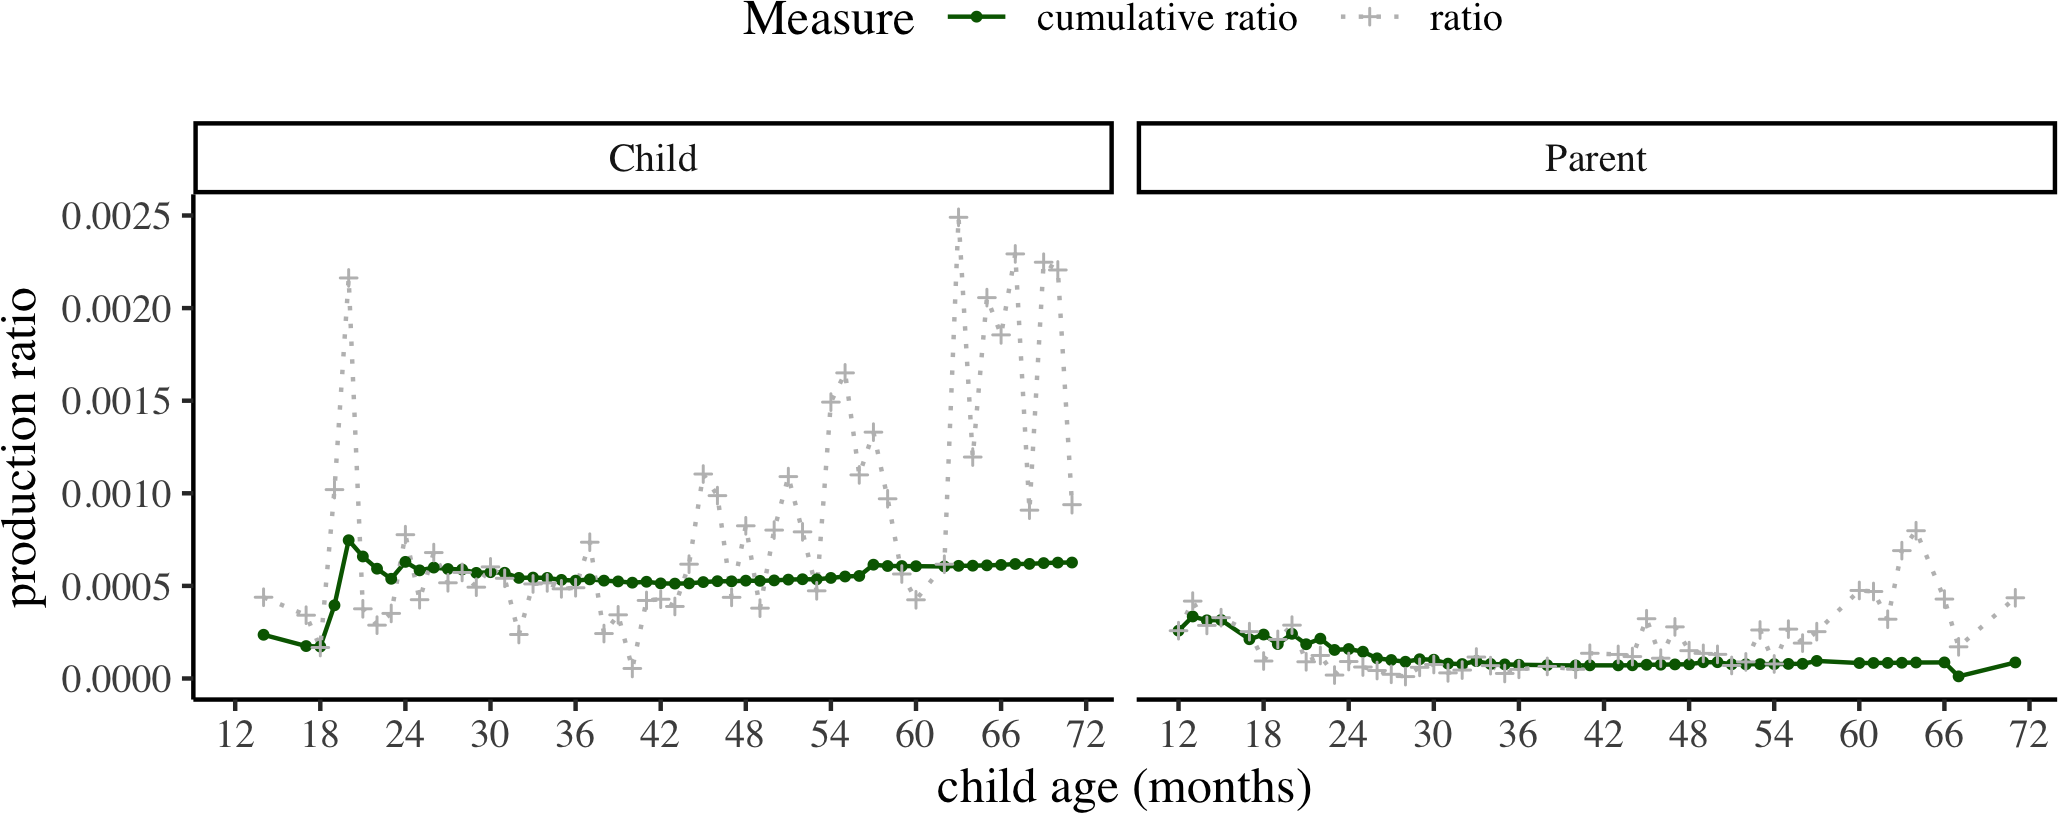
\includegraphics{neg_construction_article_files/figure-latex/prohibitiondiscourse-1} 

}

\caption{Discourse-level Prohibition.}\label{fig:prohibitiondiscourse}
\end{figure}

\hypertarget{inability}{%
\subsubsection{Inability}\label{inability}}

For the function of inability, we analyzed instances with head verbs that are modified by the modal auxiliaries \emph{can} and \emph{could}. If the head verb was also modified by a negative morpheme, we classified it as negative. Otherwise, we considered it positive. Cases without a subject (e.g.~``can't play'') or with subjects that were not first person singular (e.g.~``you can't do that,'' ``this can't go in the box'') were excluded. This is because such cases often yield readings other than ``(in)ability.'' Depending on the larger context, they could be deontic (e.g.~``you are not allowed to do that'') or epistemic (e.g.~``it is not possible for it to go in the box''). To avoid this ambiguity and focus more on constructions that convey an individual's ability, we restricted our analyses only to cases with the first person singular subject \emph{I}. This led to 7,115 negative utterances (child: 3,917; parent: 3,198), and 14,433 positive utterances (child: 7,589; parent: 6,844). Table \ref{tab:inab} shows a few example of the cases we considered.

\begin{longtable}[]{@{}ll@{}}
\caption{\label{tab:inab} Examples of constructions that convey ability and inability in children's speech at the sentence level}\tabularnewline
\toprule
Inability (Negative) & Ability (Positive) \\
\midrule
\endfirsthead
\toprule
Inability (Negative) & Ability (Positive) \\
\midrule
\endhead
\emph{I can't see} & \emph{You could do it} \\
\bottomrule
\end{longtable}

Figure \ref{fig:inability} shows ratios and cumulative ratios of parents and children's productions of inability constructions as defined above. Similar to previous constructions, positive instances are generally more frequent than negative ones. Children produce inability negation more and more frequently between 18-36 months. After 36 months, their productions are stable and close to parent ratios.

\begin{figure}[H]

{\centering 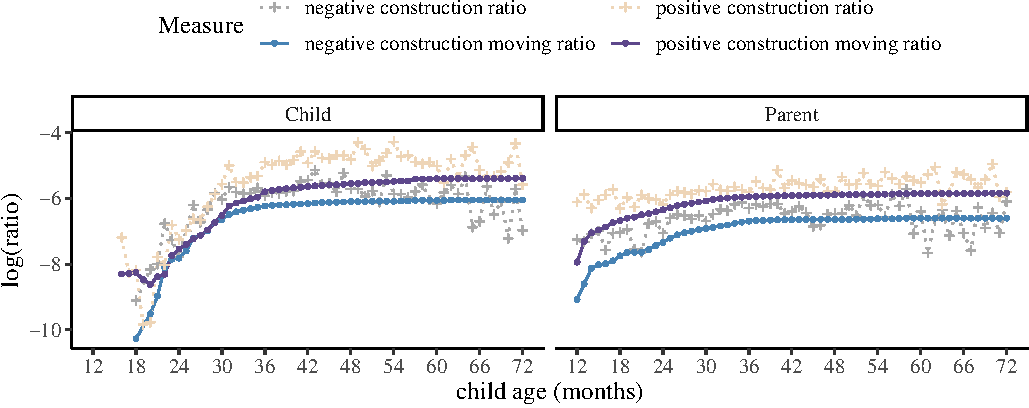
\includegraphics{neg_construction_article_files/figure-latex/inability-1} 

}

\caption{Ratios and Cumulative Ratios for parents and children's productions of the inability construction and its positive counterpart.}\label{fig:inability}
\end{figure}

At the discourse level, we selected utterances with the negative particle \emph{no} in response to antecedents that had a similar structure to the inability construction defined above. This yielded a total of 313 negative utterances (child: 11,506; parent: 10,042). Figure \ref{fig:inabilitydiscourse} shows the ratios and the moving ratios for parents' and children's production of discourse level inability construction. Considering cumulative ratios, children's productions gradually increase from 24 to 36 months and stabalizes after 36 months at a similar rate to that of parent's.

\begin{figure}[H]

{\centering 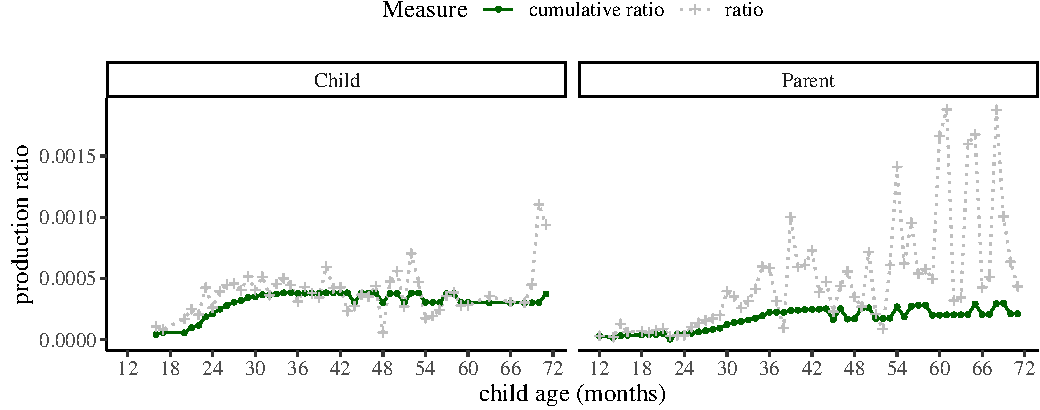
\includegraphics{neg_construction_article_files/figure-latex/inabilitydiscourse-1} 

}

\caption{Discourse-level Inability.}\label{fig:inabilitydiscourse}
\end{figure}

\hypertarget{labeling}{%
\subsubsection{Labeling}\label{labeling}}

To capture the function of labeling at the sentence level, we concentrated on copula structures in which the predicate is a nominal or an adjectival phrase. Specifically, the nominal predicates exclude possessive pronouns in order to not overlap with the communicative function of possession (see below). We considered instances where the predicate is modified by negative morphemes as negative, and others as positive. To also avoid overlap with cases of non-existence, none of the utterances contained expletives (e.g.~``there is no book''). This resulted in a total of 36,410 negative utterances (Child: 6,193; Parent: 30,217), and 484,679 positive utterances (Child: 121,107; Parent: 363,572).

\begin{longtable}[]{@{}ll@{}}
\caption{\label{tab:label} Examples of the labeling construction in children's speech at the sentence level}\tabularnewline
\toprule
Labeling (Negative) & Labeling (Positive) \\
\midrule
\endfirsthead
\toprule
Labeling (Negative) & Labeling (Positive) \\
\midrule
\endhead
\emph{that's not a farmer} & \emph{this is a book} \\
\emph{I'm not a heavy baby Mum} & \emph{it's a nice bowl} \\
\emph{It's no good} & \emph{she's pretty} \\
\bottomrule
\end{longtable}

Figure \ref{fig:learning} shows ratios and cumulative ratios for parent's and children's production of the labeling construction at the sentence level. In both parents and children, the frequency of positive counterparts is consistently higher than that of negative labeling instances. Children's productions of negative labeling increased between 18-36 months, and remained stable and close to the parent ratios after 36 months.

\begin{figure}[H]

{\centering 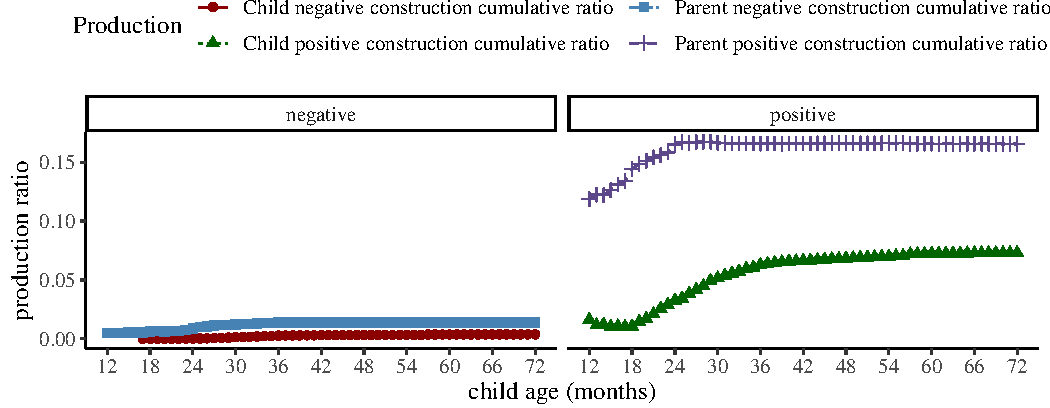
\includegraphics{neg_construction_article_files/figure-latex/learning-1} 

}

\caption{Ratios and cumulative ratios for instances of (negative) labeling and its positive counterparts in parents' and children's speech.}\label{fig:learning}
\end{figure}

At the discourse level, we selected antecedent utterances with copula structures that combined with a nominal or an adjectival predicate. Table \ref{tab:dislabel} shows a few examples. We found 4,079 utterances (Child: 2,234; Parent: 1,845). Figure \ref{fig:learningdiscourse} shows the log ratios and cumulative ratios for labeling instances at the discourse level. Children used negation to respond to labeling utterances more frequently between 18 to 30 months. After 30 months, children's productions of negative labeling continues to increase but remains close to parents' level more generally.

\begin{longtable}[]{@{}ll@{}}
\caption{\label{tab:dislabel} Example antecedent labeling and discourse level negation in parents' and children's productions}\tabularnewline
\toprule
Antecedent & Utterance \\
\midrule
\endfirsthead
\toprule
Antecedent & Utterance \\
\midrule
\endhead
Child: \emph{that's the one} & Parent: \emph{no it's the green one} \\
\bottomrule
\end{longtable}

\begin{figure}[H]

{\centering 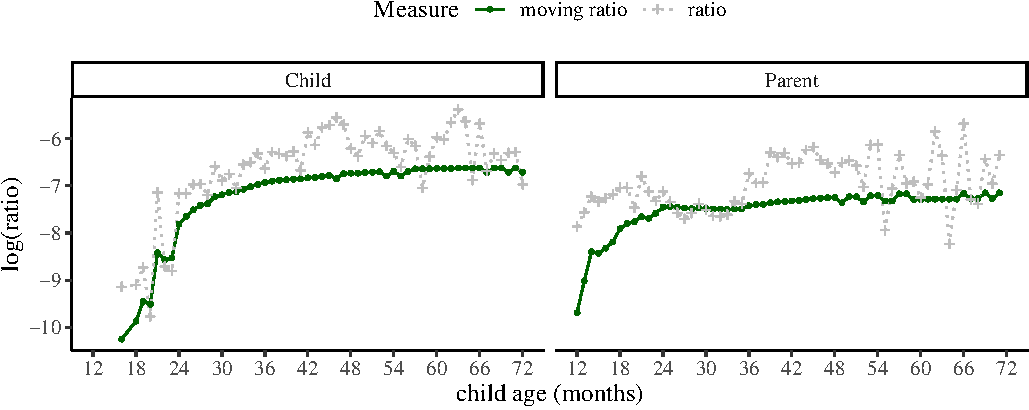
\includegraphics{neg_construction_article_files/figure-latex/learningdiscourse-1} 

}

\caption{Log ratios and cumulative ratios of discourse level labeling instances in parents' and children's productions.}\label{fig:learningdiscourse}
\end{figure}

\hypertarget{epistemic-negation}{%
\subsubsection{Epistemic Negation}\label{epistemic-negation}}

Previous studies have reported instances in which children combined negative morphemes with mental state verbs such as \emph{know}, \emph{think}, and \emph{remember} to express ``epistemic negation'' (Choi, 1988). For defining epistemic constructions we also focused on these three verbs. For sentence level epistemic negation, we analyzed negative utterances where these verbs were modified by negative morphemes, possibly after combining with an auxiliary verb like \emph{do}. Table \ref{tab:epistem} shows a few examples. Instances where the speaker asked about or describes the negative epistemic state of another speaker were also included, leading to 31,696 negative utterances in total (child: 9,852; parent: 21,844). For the positive counterparts, we selected instances with the same head verbs except that these verbs were not modified by negation. This resulted in a total of 95,679 negative utterances (child: 16,322; parent: 79,357).

\begin{longtable}[]{@{}ll@{}}
\caption{\label{tab:epistem} Examples of the epistemic construction in children's speech at the sentence level}\tabularnewline
\toprule
Epistemic (Negative) & Epistemic (Positive) \\
\midrule
\endfirsthead
\toprule
Epistemic (Negative) & Epistemic (Positive) \\
\midrule
\endhead
\emph{I not know} & \emph{I knows} \\
\emph{I didn't remember} & \\
\emph{I don't think so} & \emph{I think this one is good} \\
\emph{don't you remember} & \\
\emph{She doesn't know this} & \emph{She knows about this} \\
\bottomrule
\end{longtable}

Figure \ref{fig:epistemic} shows log ratios and cumulative ratios of the epistemic construction as defined above in parents' and children's speech at the sentence level. Overall, positive epistemic utterances were more frequent than negative epistemic utterances, with the possible exception of \emph{know} for children. The production of negative utterances headed by \emph{know} was comparatively the highest among children, and became more frequent at an earlier age (17-18 months) compared to that of \emph{remember} (\textasciitilde19 months) or \emph{think} (\textasciitilde20 months). Across the three head verbs, children's productions with \emph{know} and \emph{remember} gradually approaches that of parents' around 30 - 36 months, whereas cases with the head verb \emph{think} tend to be produced less frequently by children.

\begin{figure}[H]

{\centering 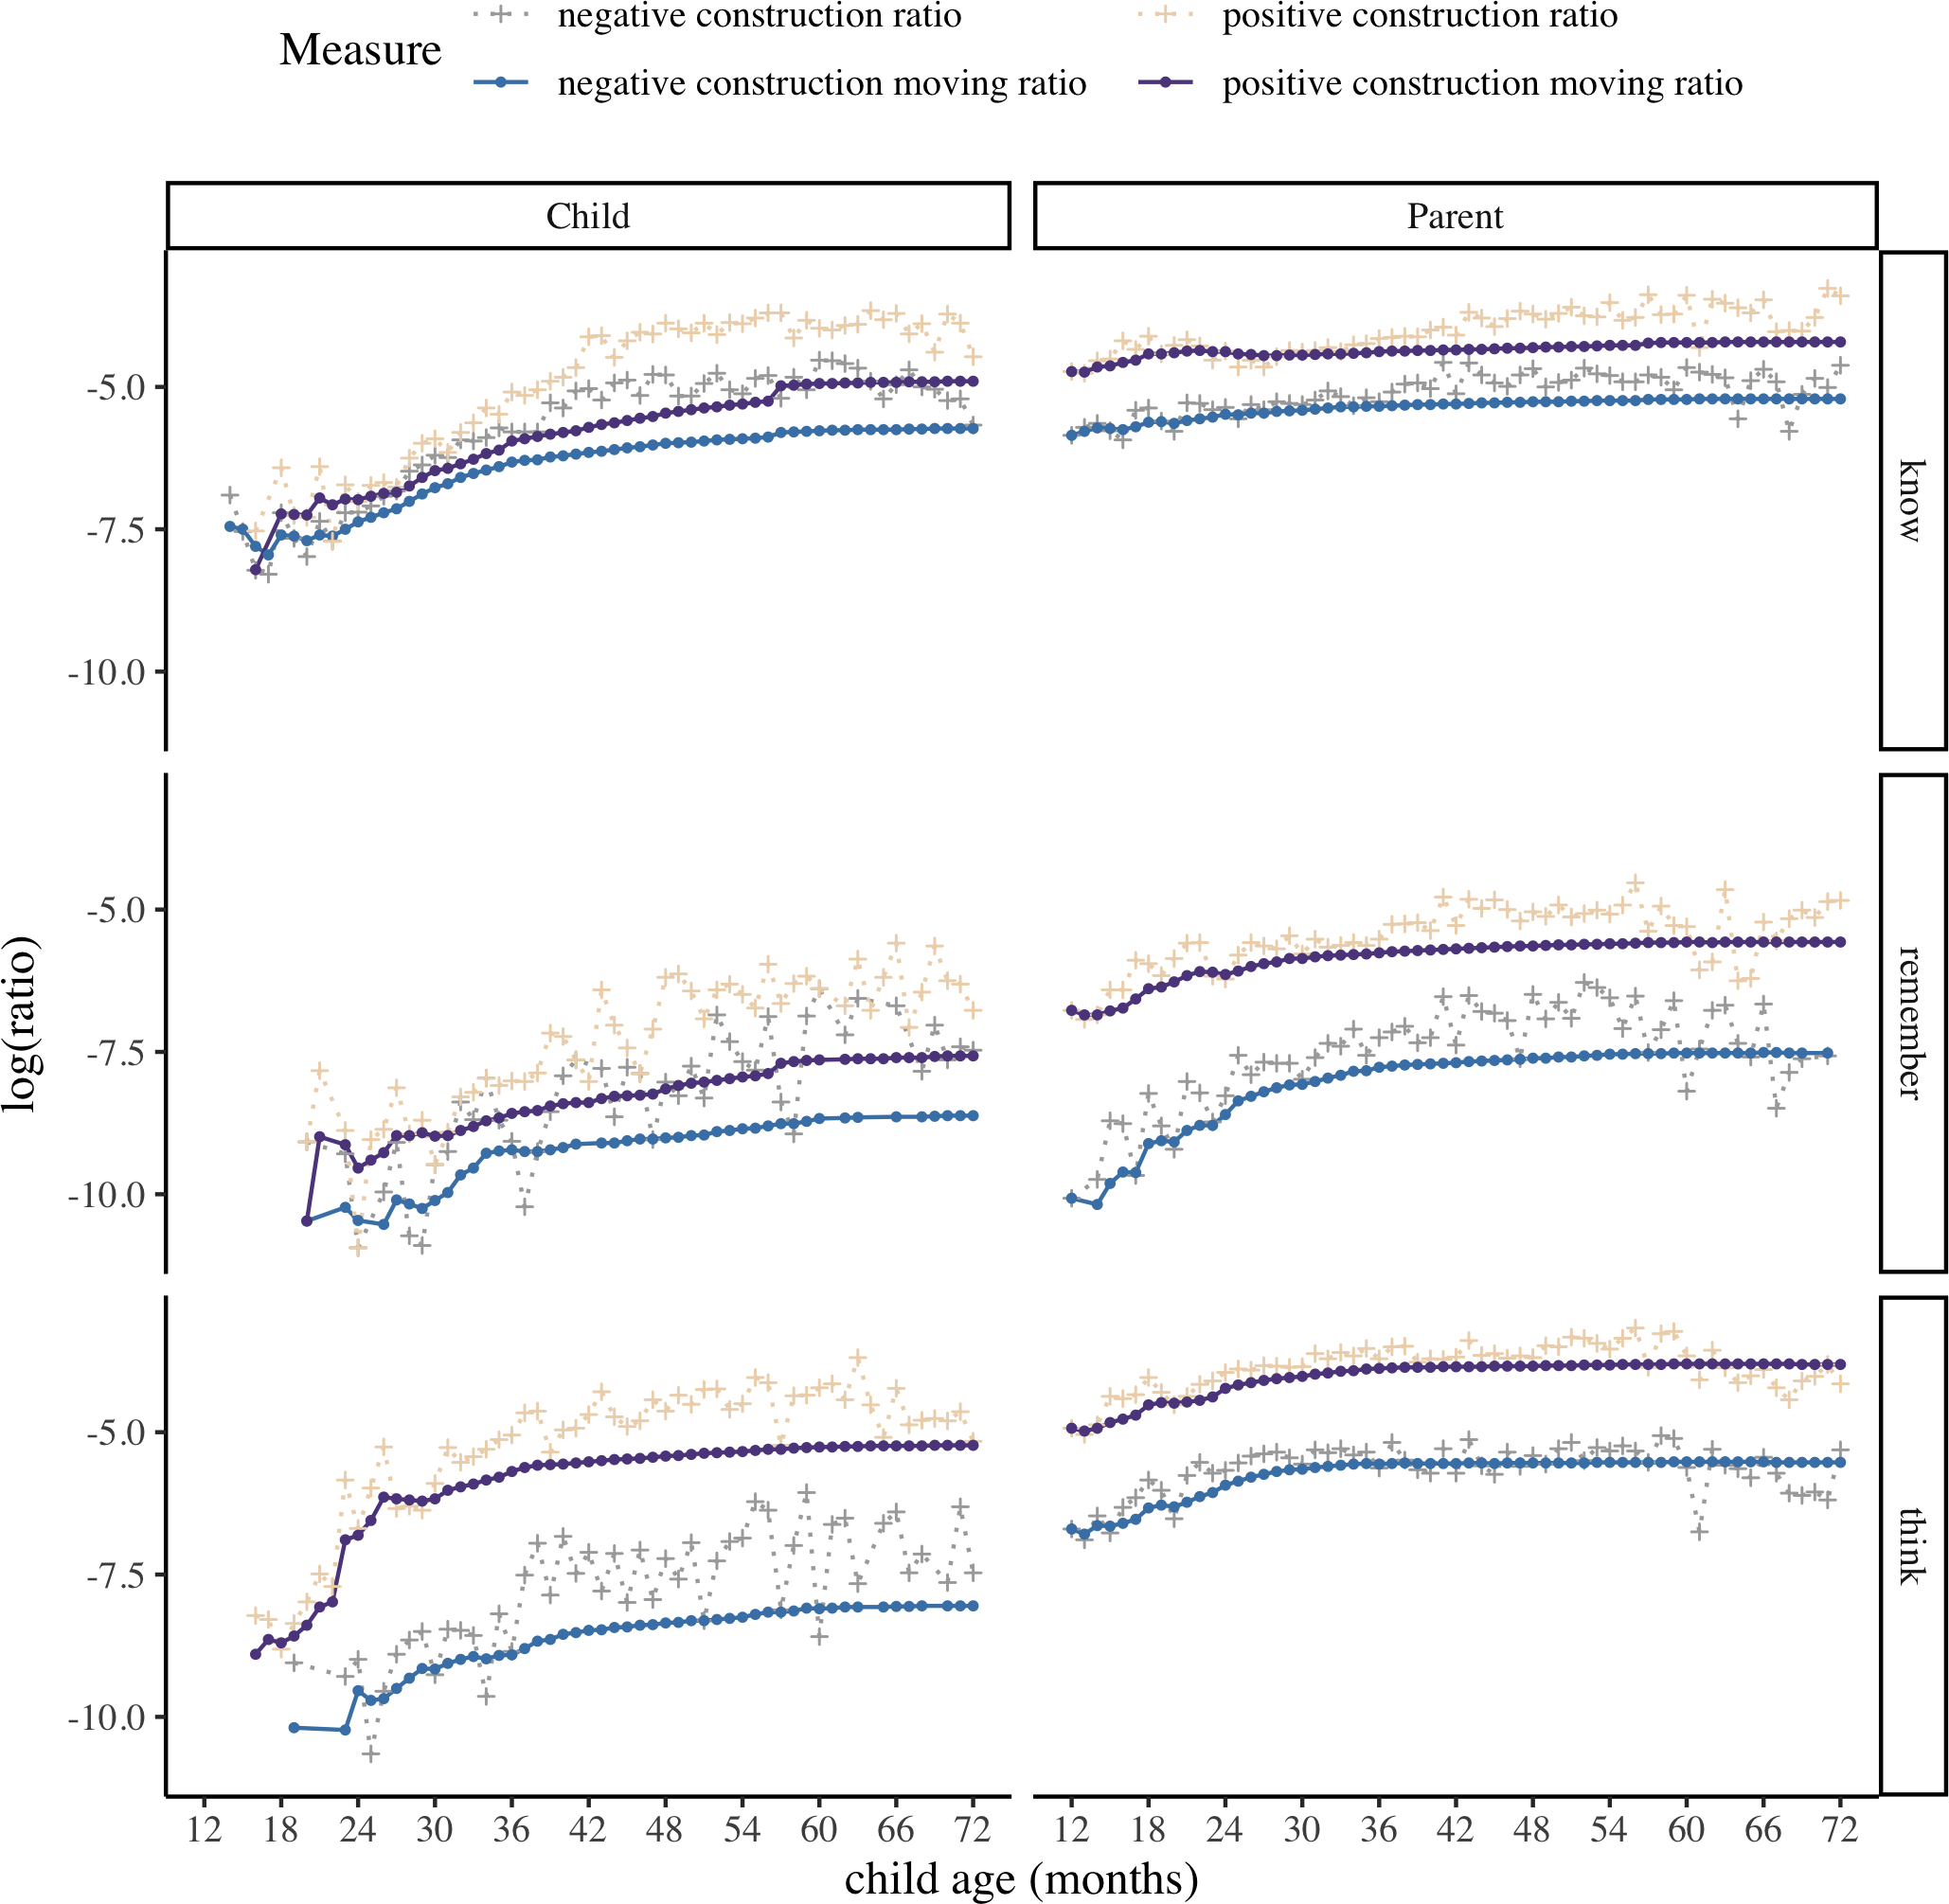
\includegraphics{neg_construction_article_files/figure-latex/epistemic-1} 

}

\caption{Log ratios and cumulative ratios of negative and positive epistemic utterances in parents' and children's speech.}\label{fig:epistemic}
\end{figure}

For epistemic negation at the discourse level, we examined interactions in which the antecedent utterances took any of the three head verbs \emph{know}, \emph{remember} and \emph{think}, leading to a total of 985 utterances (child: 26,174; parent: 101,201). Figure \ref{fig:epistemicdiscourse} shows log ratios and cumulative ratios for epistemic negation at the discourse level. Children's productions increase rapidly between 24-36 months and after 36 months, they produce this construction close to parent levels.

\begin{figure}[H]

{\centering 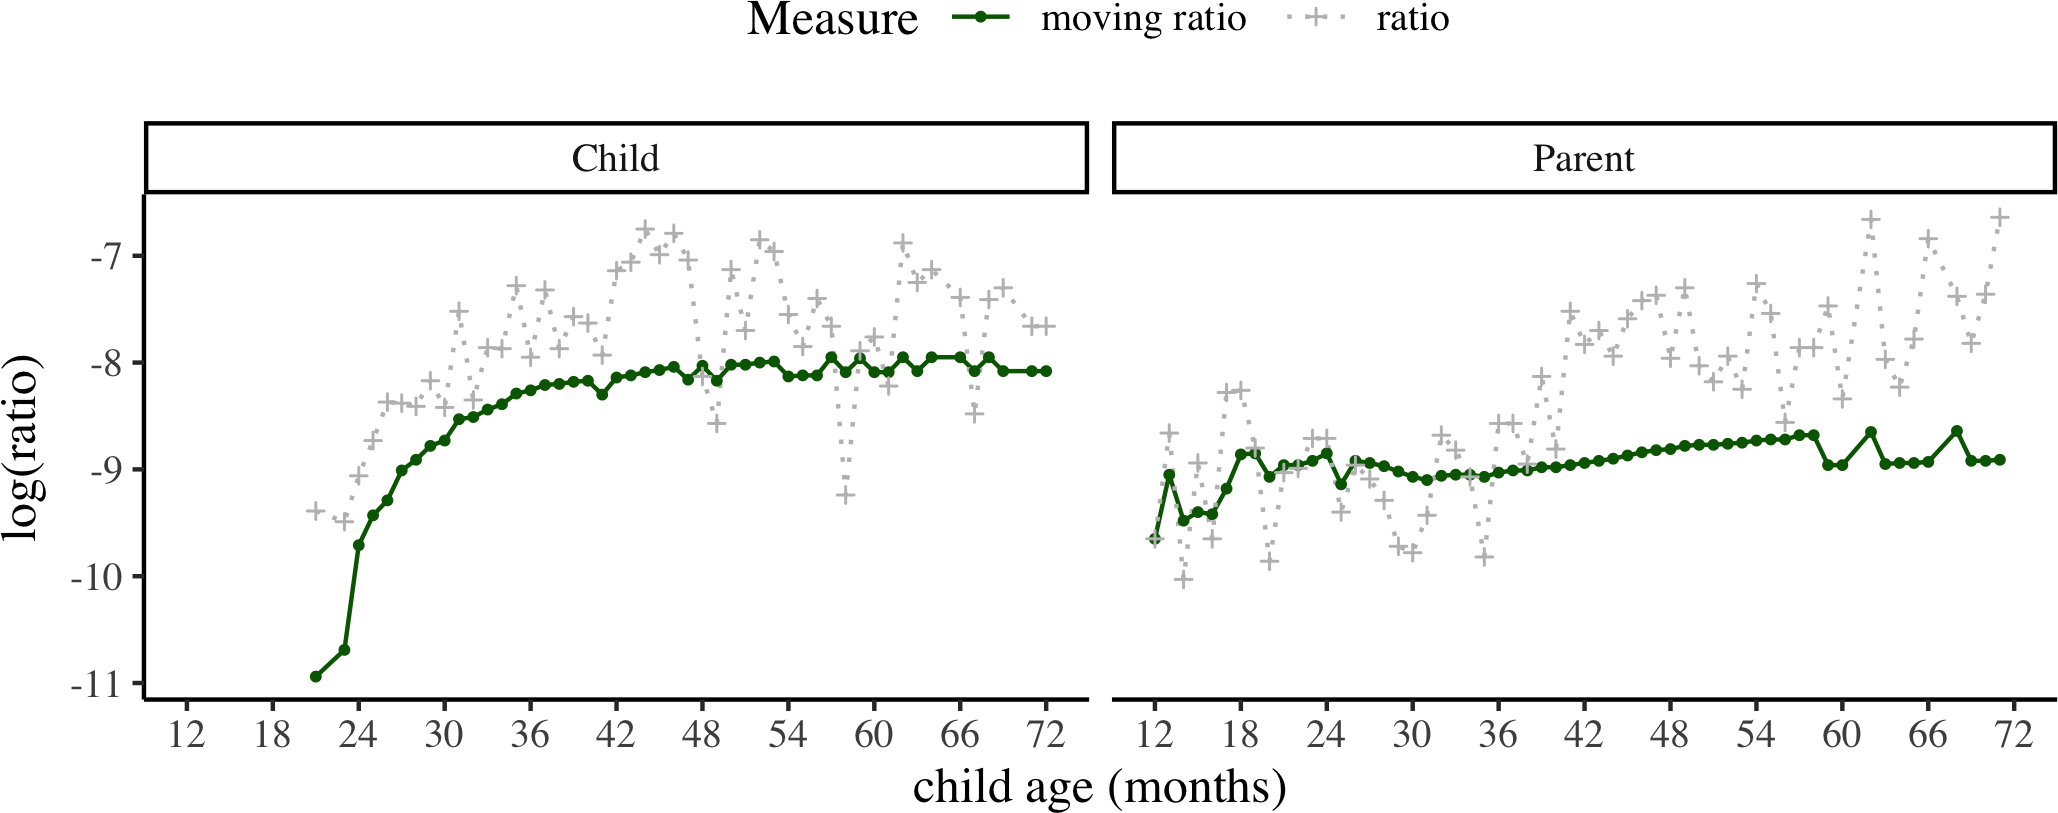
\includegraphics{neg_construction_article_files/figure-latex/epistemicdiscourse-1} 

}

\caption{Log ratios and cumulative ratios for discourse level Epistemic negation in parents' and children's speech.}\label{fig:epistemicdiscourse}
\end{figure}

\hypertarget{possession}{%
\subsubsection{Possession}\label{possession}}

The last function we explored was ``possession.'' At the syntactic level, for negative structures we selected cases where negative morphemes were combined with auxiliary verbs to modify a head verb with the lemma form \emph{have} and a POS tag of VERB. We also included individual noun phrases with possessive pronouns as heads and modified by negative morphemes. Table \ref{tab:possess} shows a few examples. Cases in which the syntactic head of the negative morphemes is a predicate of a copula verb (e.g.~``this is not mine'') were excluded to separate them from the function ``labeling.'' The number of negative utterances that were subjected to analysis for this function is 8,892 (child: 2,830; parent: 6,062). Again the positive counterparts share similar structures except with no negation, leading to a total of 86,665 (child: 27,730; parent: 58,935). One thing to note here is that for the positive structures with the head verb \emph{have}, we restricted to cases where the verb takes a direct object (with the dependency relation \emph{obj}). This is to avoid potential parsing errors of instances such as \emph{I have}, where the verb could ambiguously be an auxiliary.

\begin{longtable}[]{@{}ll@{}}
\caption{\label{tab:possess} Examples of negative and positive possession in children and parents' speech at the sentence level}\tabularnewline
\toprule
Posession (Negative) & Posession (Positive) \\
\midrule
\endfirsthead
\toprule
Posession (Negative) & Posession (Positive) \\
\midrule
\endhead
\emph{I don't have it} & \emph{you have that} \\
\emph{not mine} & \emph{hers} \\
\bottomrule
\end{longtable}

Figure \ref{fig:possession} shows log ratios and cumulative ratios of the negative and positive possession construction at the sentence level. The production trajectory for possession in child speech appears to have notable differences depending on what the negative morpheme modifies. With \emph{have} as the syntactic head, children increase their productions between 18-36 months, and stay close to parent levels of production after 36 months. However, for utterances headed by possessive pronouns, productions increase rapidly between 18-24 months and stays close to parent levels as early as 24 months of age.

\begin{figure}[H]

{\centering 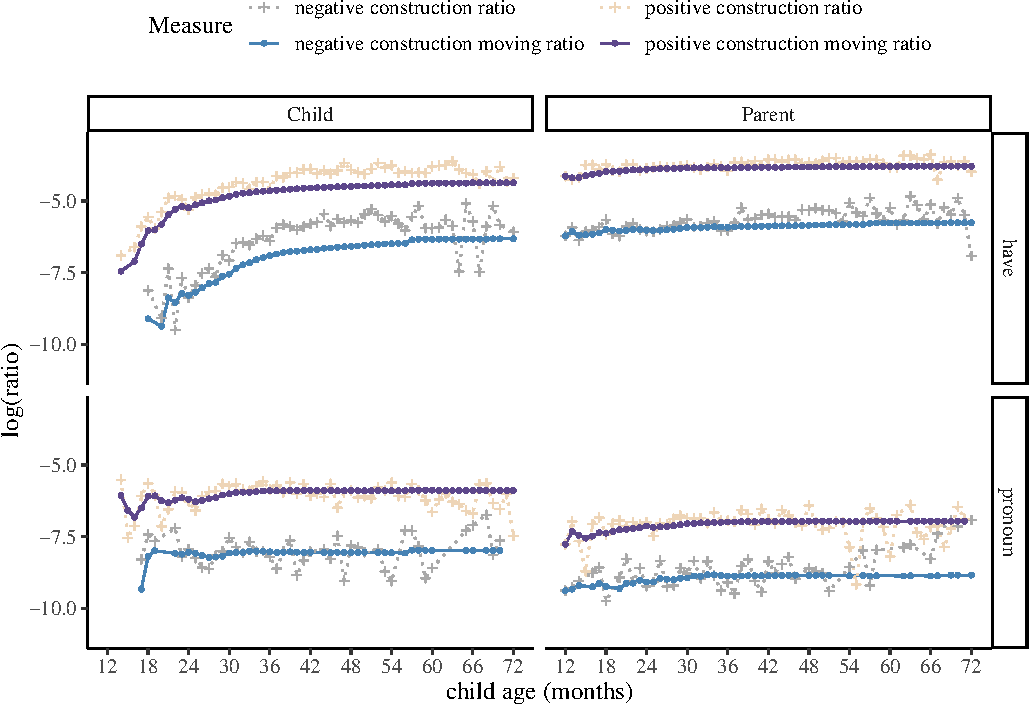
\includegraphics{neg_construction_article_files/figure-latex/possession-1} 

}

\caption{Log ratios and cumulative ratios of the construction `possession` in parents' and children's speech.}\label{fig:possession}
\end{figure}

At the discourse level, we selected antecedents to discourse level negative utterances (e.g.~\emph{no!}) which themselves had structures similar to both the negative and positive constructions at the syntactic level. Table \ref{tab:dispossess} provides a few examples and Figure \ref{fig:possessiondiscourse} shows log ratios and cumulative ratios of such utterances in parents' and children's speech. Overall, the production pattern for discourse level possession suggests that children produce such utterances frequently and at parents' level after 30 or 36 months of age.

\begin{longtable}[]{@{}ll@{}}
\caption{\label{tab:dispossess} Example antecedents with the possession construction and discourse level negation in parents' and children's productions}\tabularnewline
\toprule
Antecedent & Utterance \\
\midrule
\endfirsthead
\toprule
Antecedent & Utterance \\
\midrule
\endhead
Child: \emph{I don't have the book} & Parent: \emph{no no mommy please read it to me} \\
Parent: \emph{not yours} & Child: \emph{no it's mine mine} \\
\bottomrule
\end{longtable}

\begin{figure}[H]

{\centering 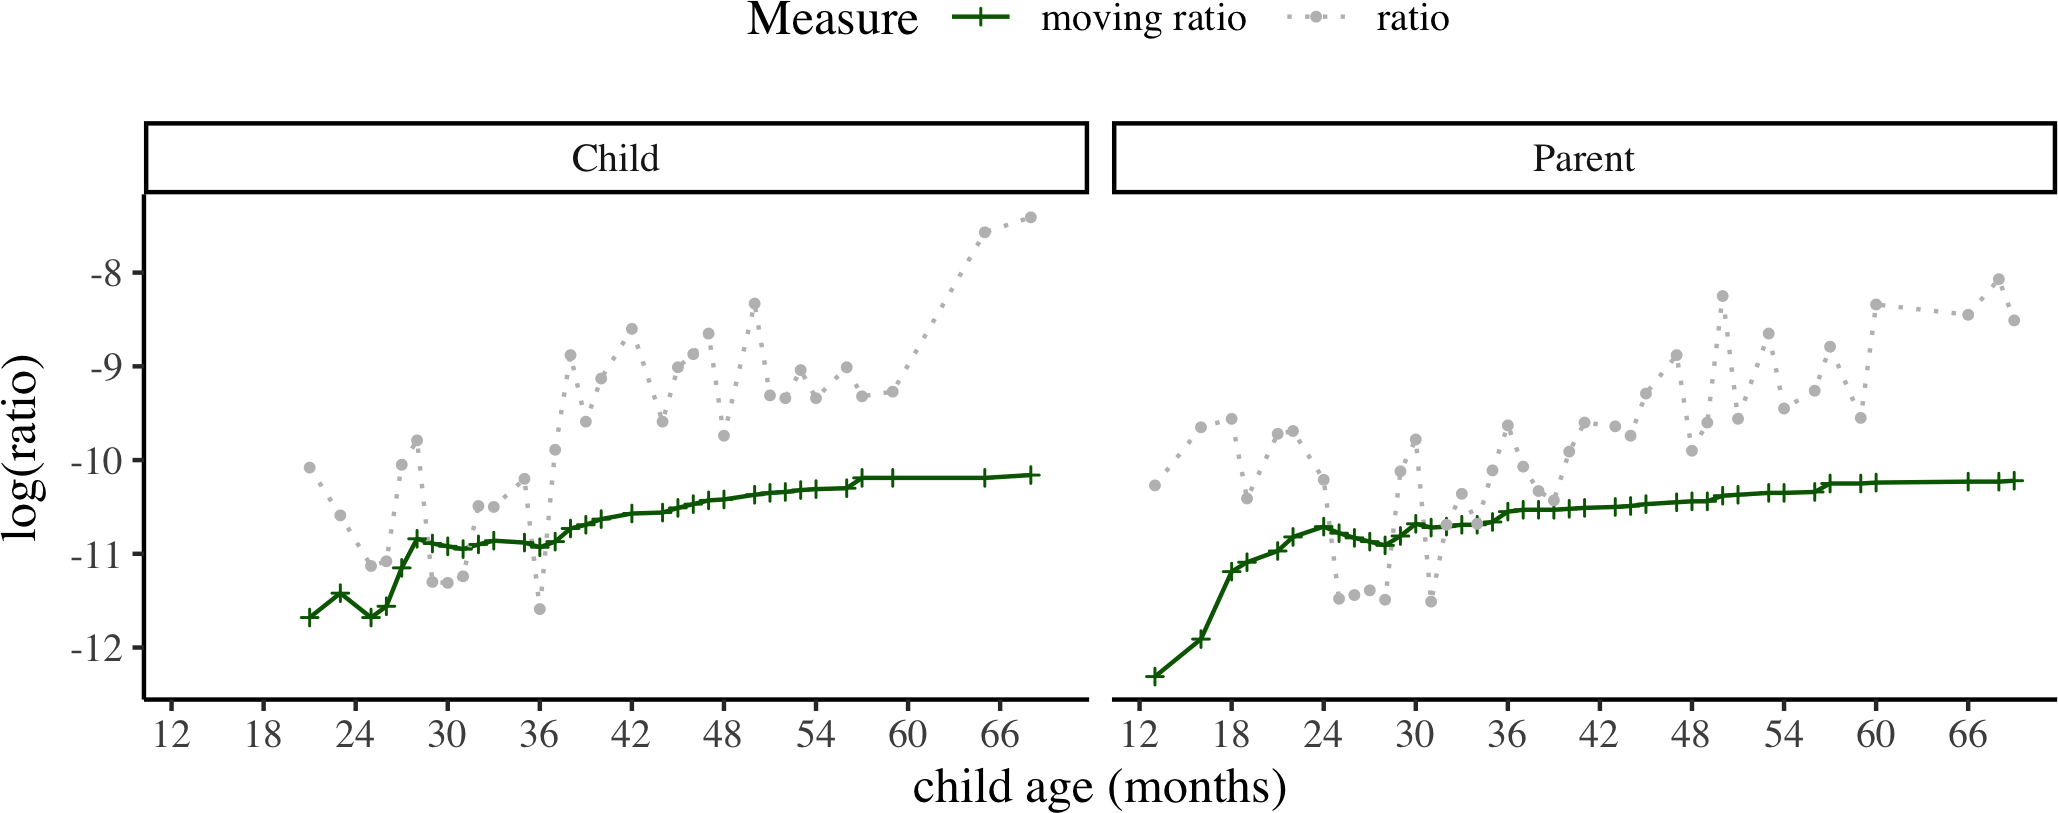
\includegraphics{neg_construction_article_files/figure-latex/possessiondiscourse-1} 

}

\caption{Log ratios and cumulative ratios of the possession construction at the discourse level in parents' and children's speech.}\label{fig:possessiondiscourse}
\end{figure}

\hypertarget{discussion}{%
\subsubsection{Discussion}\label{discussion}}

\begin{figure}[H]

{\centering 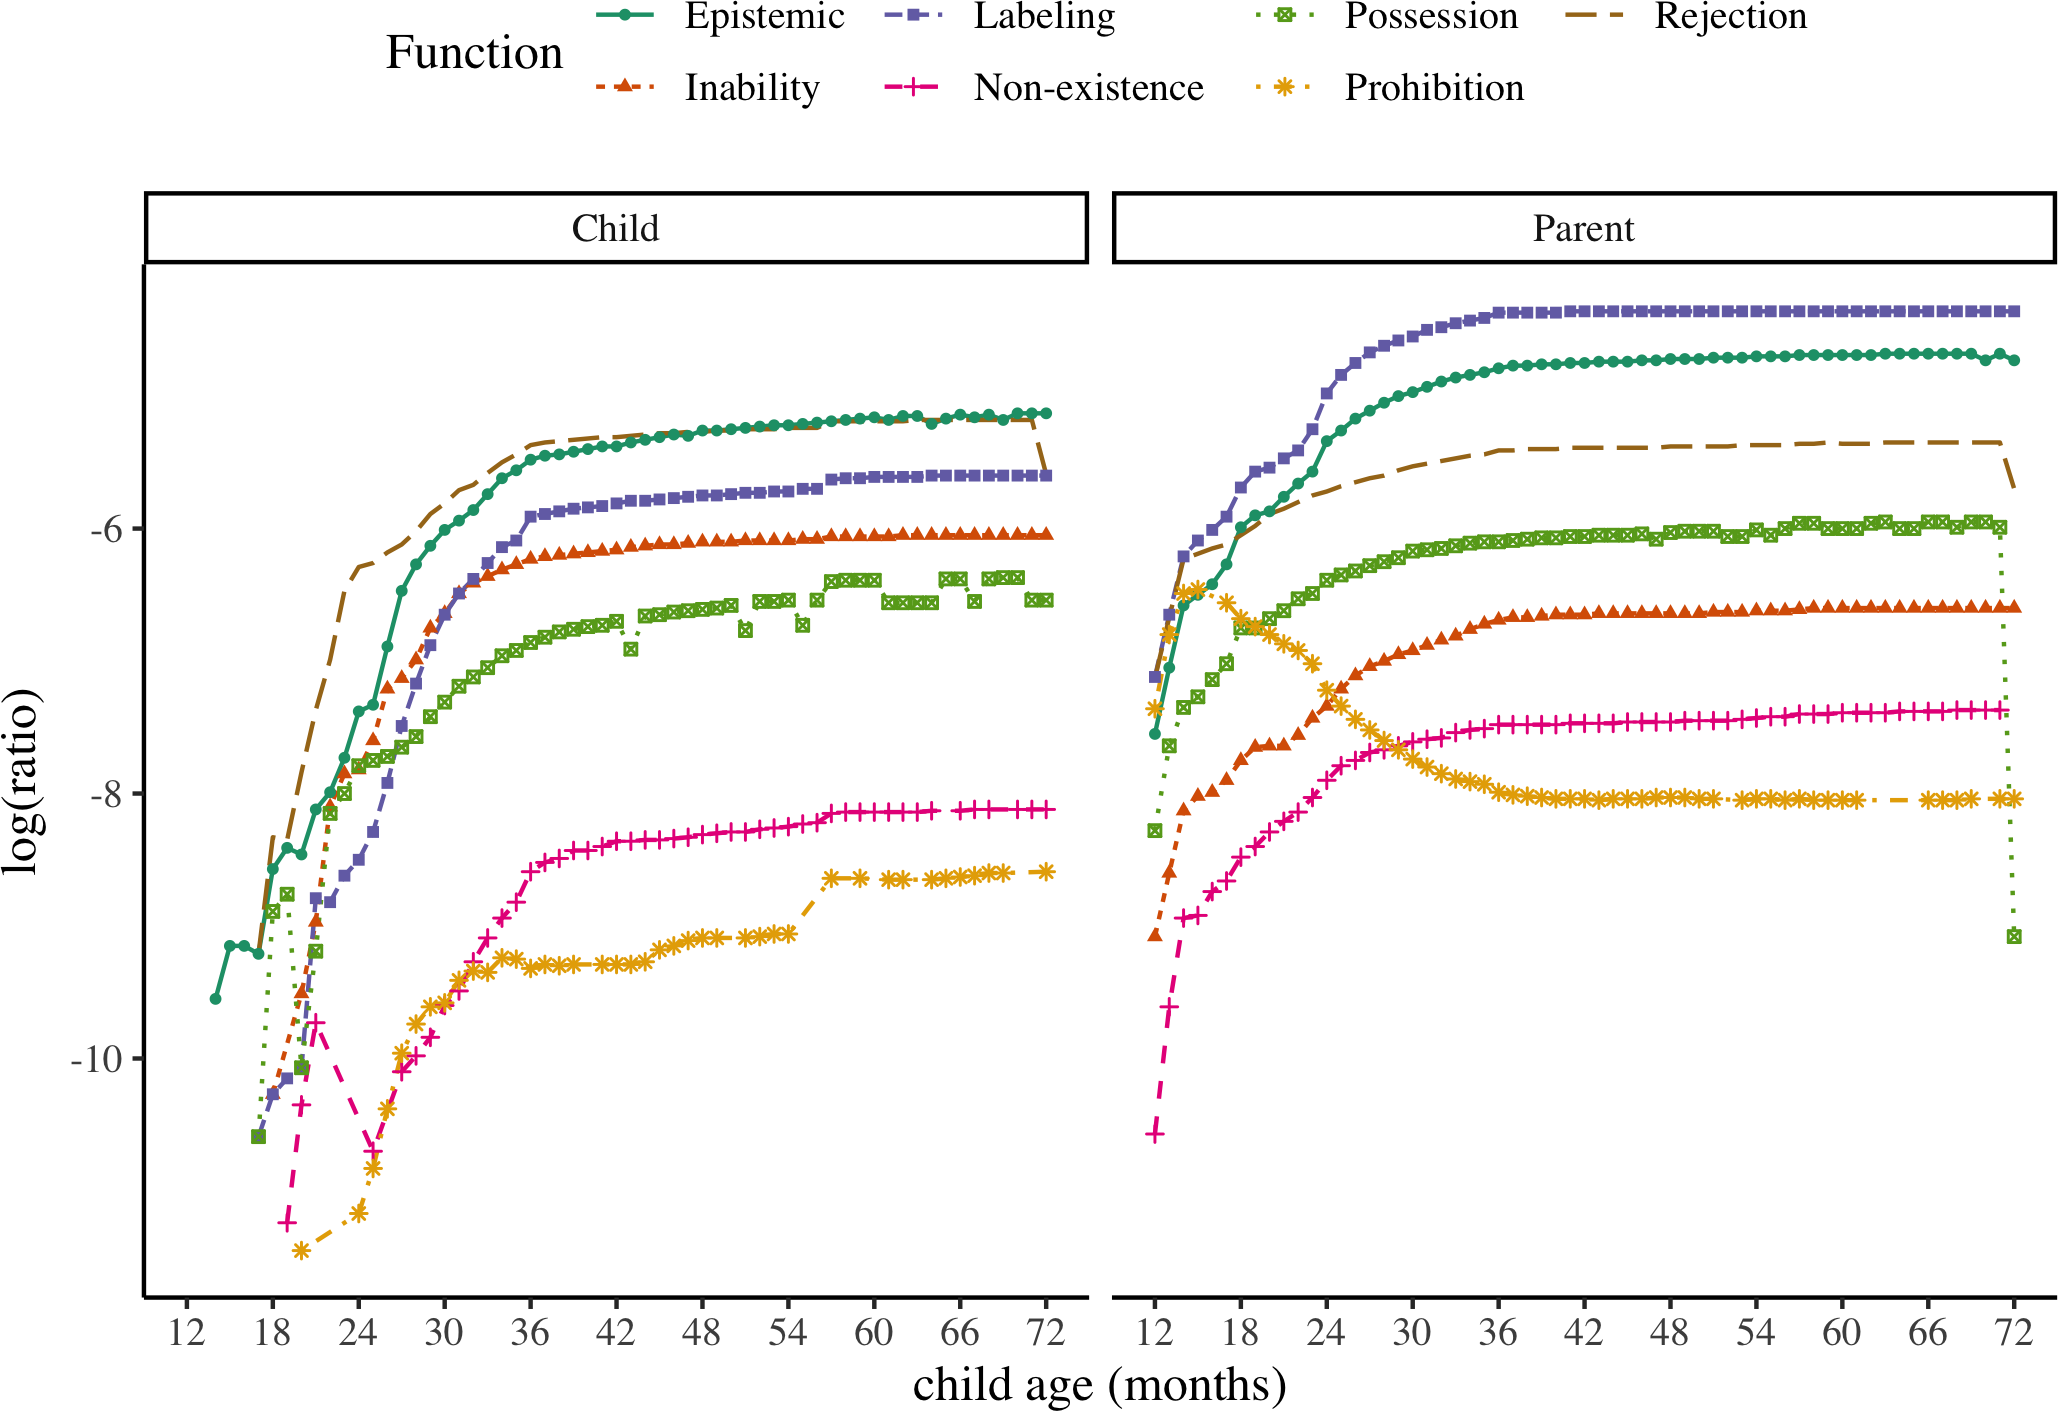
\includegraphics{neg_construction_article_files/figure-latex/allneg-1} 

}

\caption{Log cumulative ratios for all negative constructions at the syntactic level.}\label{fig:allneg}
\end{figure}

\begin{figure}[H]

{\centering 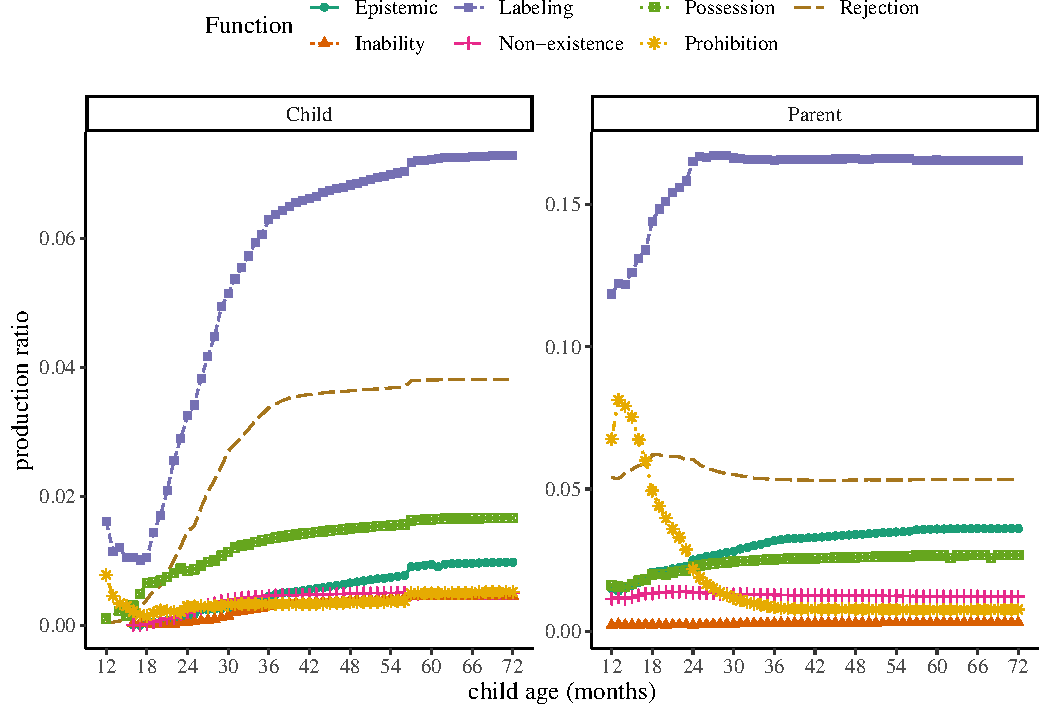
\includegraphics{neg_construction_article_files/figure-latex/allpos-1} 

}

\caption{Log cumulative ratios for the positive counpterparts to all negative constructions at the syntactic level.}\label{fig:allpos}
\end{figure}

\begin{figure}[H]

{\centering 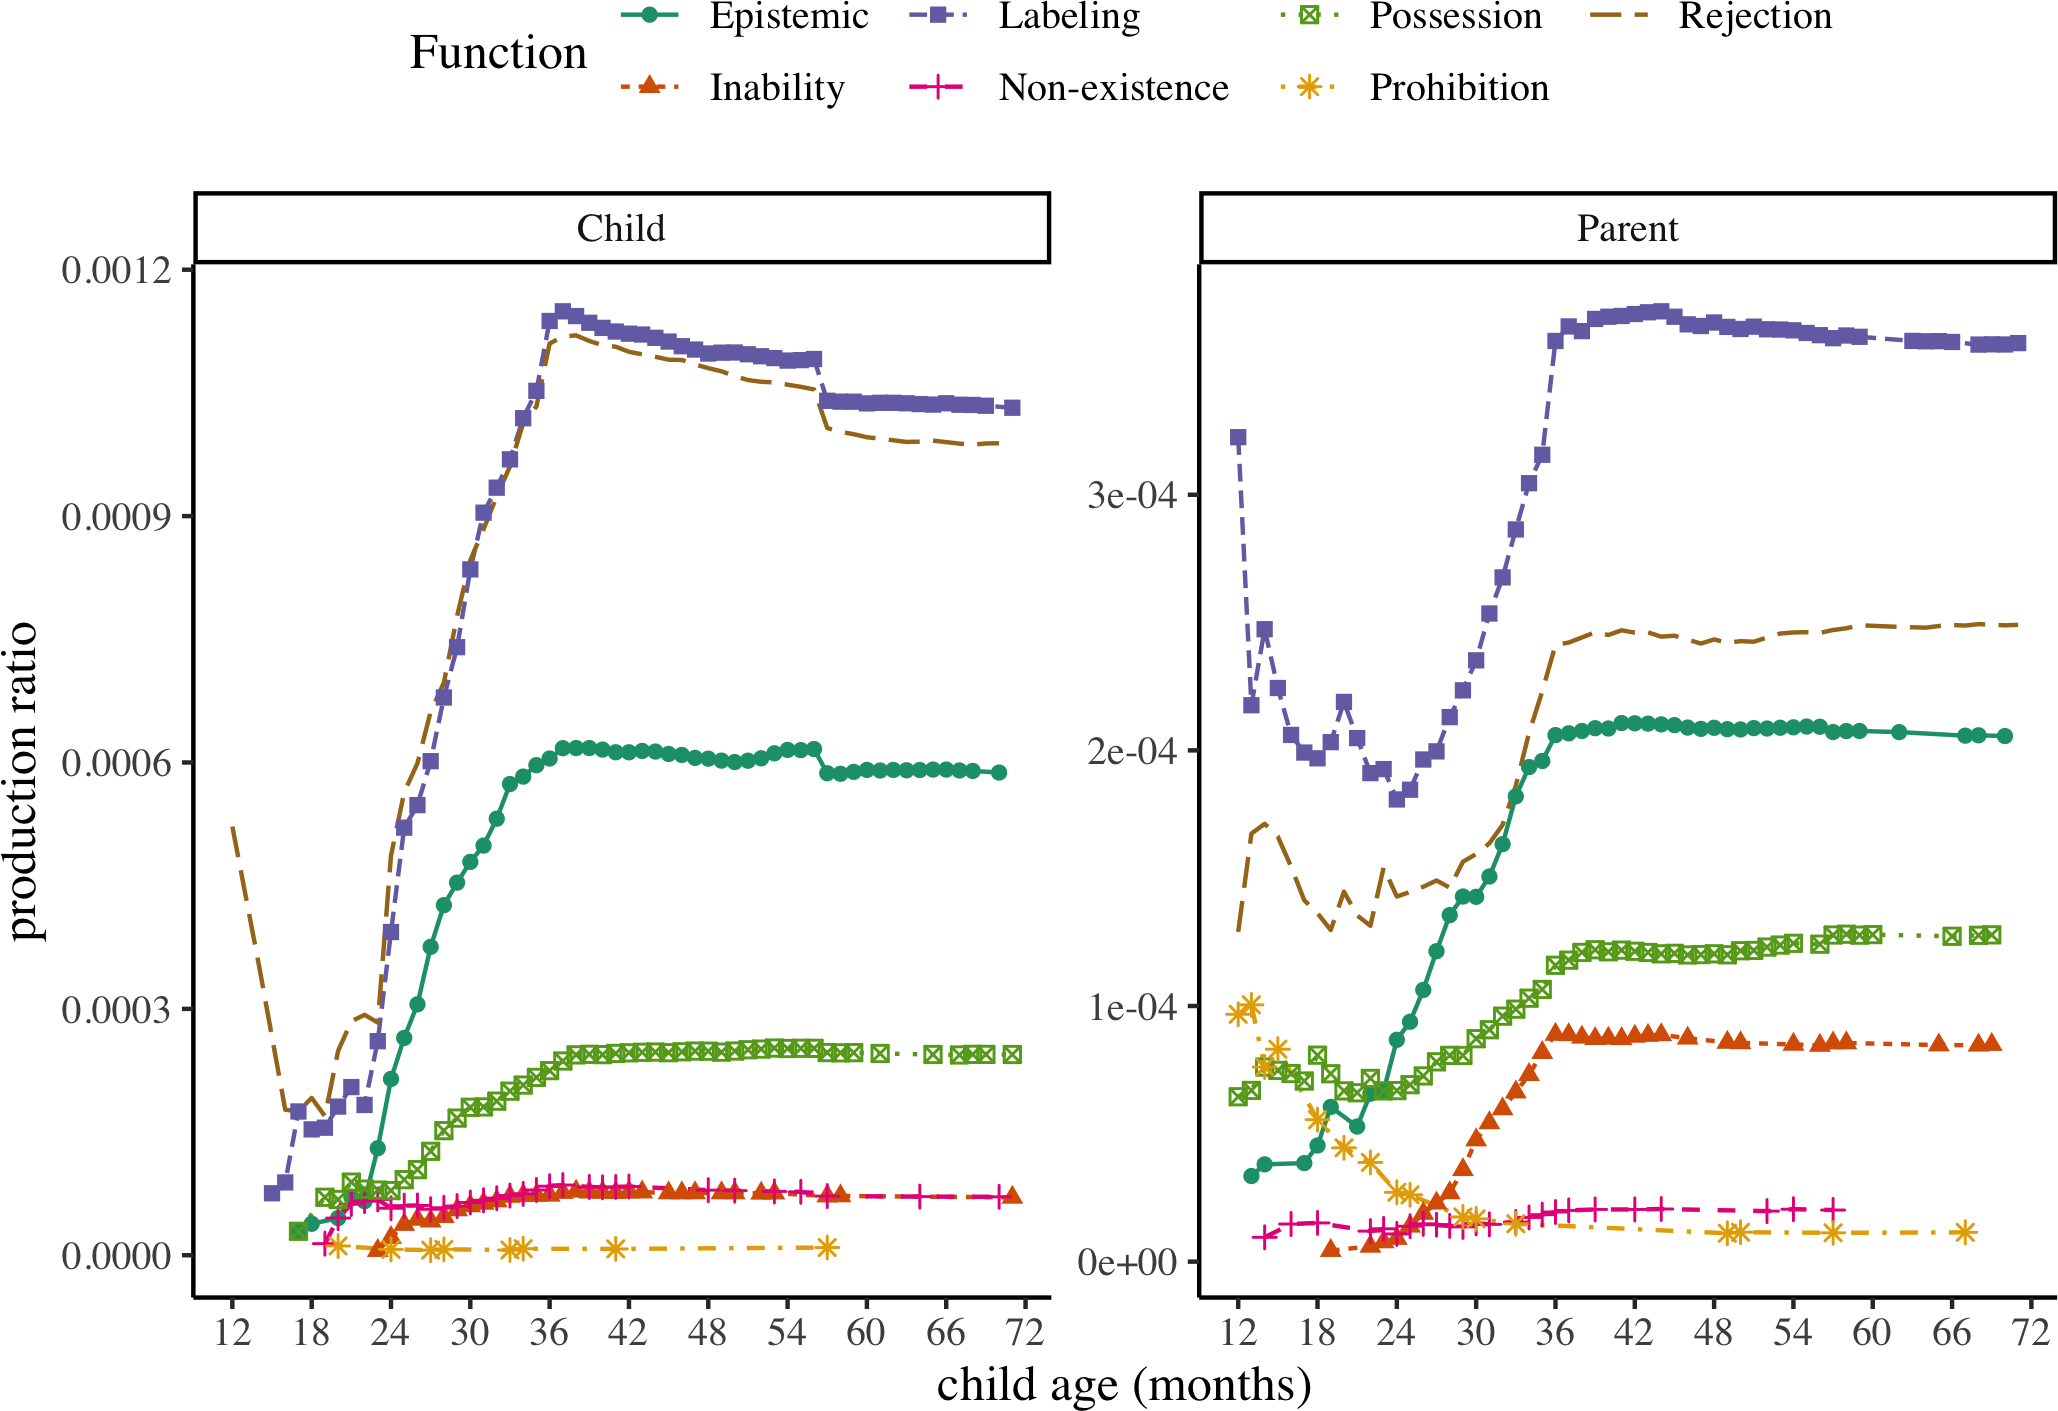
\includegraphics{neg_construction_article_files/figure-latex/alldiscourse-1} 

}

\caption{Cumulative ratios for all negative constructions at the discourse level.}\label{fig:alldiscourse}
\end{figure}

\hypertarget{conclusion}{%
\section{Conclusion}\label{conclusion}}

Using automatic annotations of large-scale corpora of child-parent interactions, we presented production trajectories for seven negative constructions that tend to express rejection, non-existence, prohibition, inability, labeling, epistemic states, and possession (Table 1). The results suggest that the production of almost all these negative constructions (except for prohibition) emerges and gradually increases within the 18-36 months age range (Figure 8). Their production frequencies remain stable and regular after 36 months and relatively close to parents' levels of production. It is important to note that similar to prior studies, our conclusions are limited to negation in children's production. Systematic experiments testing children's comprehension of negative utterances with different communicative functions are necessary to better understand the origins and developmental trajectory of negation.

For future work, we would like to explore several directions. First, to more thoroughly examine and potentially model the developmental trajectories of negation in child production, certain production-specific factors (e.g.~length of utterance, ease of pronunciation) should be taken into account as well. In addition, we aim to investigate the production trajectory of positive counterparts to our negative structures (e.g.~``I know'' for ``I don't know''). Comparisons of negative utterances in relation to their positive counterparts would allow us to further analyze the developmental paths of negation within specific constructions.

Lastly, our experiments have concentrated on larger syntactic structures at the utterance level, hence cases where negation is used as discourse markers to respond to previous utterance(s) were excluded. However, these instances also have important semantic and conceptual roles in the communication between children and parents (e.g.~parent: \emph{do you want some bread?}; child: \emph{no no no}). Thus inclusions of negative structures at a more comprehensive level would be able to paint a more clear picture about the development of negation.

\begingroup
\setlength{\parindent}{-0.5in}
\setlength{\leftskip}{0.5in}

\endgroup

\hypertarget{refs}{}
\begin{CSLReferences}{1}{0}
\leavevmode\hypertarget{ref-diaparser}{}%
Attardi, G., Sartiano, D., \& Yu, Z. (n.d.). DiaParser attentive dependency parser. \emph{Submitted for Publication}.

\leavevmode\hypertarget{ref-bloom1970language}{}%
Bloom, L. M. (1970). \emph{Language development: Form and function in emerging grammars} (PhD thesis). Columbia University.

\leavevmode\hypertarget{ref-cameron2007part}{}%
Cameron-Faulkner, T., Lieven, E., \& Theakston, A. (2007). What part of no do children not understand? A usage-based account of multiword negation. \emph{Journal of Child Language}, \emph{34}(2), 251.

\leavevmode\hypertarget{ref-choi1988semantic}{}%
Choi, S. (1988). The semantic development of negation: A cross-linguistic longitudinal study. \emph{Journal of Child Language}, \emph{15}(3), 517--531.

\leavevmode\hypertarget{ref-clark2010adult}{}%
Clark, E. V. (2010). Adult offer, word-class, and child uptake in early lexical acquisition. \emph{First Language}, \emph{30}(3-4), 250--269.

\leavevmode\hypertarget{ref-darwin1872expression}{}%
Darwin, C. (1872). \emph{The expression of the emotions in man and animals}. John Murray.

\leavevmode\hypertarget{ref-demuth2006word}{}%
Demuth, K., Culbertson, J., \& Alter, J. (2006). Word-minimality, epenthesis and coda licensing in the early acquisition of {E}nglish. \emph{Language and Speech}, \emph{49}(2), 137--173.

\leavevmode\hypertarget{ref-macwhinney2000childes}{}%
MacWhinney, B. (2000). \emph{The CHILDES project: Tools for analyzing talk. Transcription format and programs} (Vol. 1). Psychology Press.

\leavevmode\hypertarget{ref-nordmeyer2018individual}{}%
Nordmeyer, A., \& Frank, M. C. (2018). Individual variation in children's early production of negation. In \emph{Proceedings of the 40th annual meeting of the cognitive science society} (pp. 2167--2172).

\leavevmode\hypertarget{ref-pea1978}{}%
Pea, R. (1978). \emph{The development of negation in early child language} (PhD thesis). University of Oxford.

\leavevmode\hypertarget{ref-qi-etal-2020-stanza}{}%
Qi, P., Zhang, Y., Zhang, Y., Bolton, J., \& Manning, C. D. (2020). {S}tanza: A python natural language processing toolkit for many human languages, 101--108. \url{https://doi.org/10.18653/v1/2020.acl-demos.14}

\leavevmode\hypertarget{ref-sanchez2019childes}{}%
Sanchez, A., Meylan, S. C., Braginsky, M., MacDonald, K. E., Yurovsky, D., \& Frank, M. C. (2019). Childes-db: A flexible and reproducible interface to the child language data exchange system. \emph{Behavior Research Methods}, \emph{51}(4), 1928--1941.

\leavevmode\hypertarget{ref-dg}{}%
Tesnière, L. (1959). \emph{Éléments de syntaxe structurale}. Paris: Klincksieck.

\leavevmode\hypertarget{ref-de1979form}{}%
Villiers, P. A. de, \& Villiers, J. G. de. (1979). Form and function in the development of sentence negation. \emph{Papers and Reports on Child Language Development}, \emph{17}, 57--64.

\leavevmode\hypertarget{ref-wei2006time}{}%
Wei, W. W. (2006). Time series analysis. In \emph{The oxford handbook of quantitative methods in psychology: Vol. 2}.

\end{CSLReferences}


\end{document}
